\documentclass[11pt]{article}
\usepackage[margin=1in]{geometry}
\usepackage{amsmath,amssymb}
\usepackage{graphicx}
\usepackage{booktabs}
\usepackage{float}
\usepackage[font=small,labelfont=bf]{caption}
\usepackage[authoryear,round]{natbib}
\usepackage[colorlinks=true,linkcolor=blue!50!black,citecolor=blue!50!black,urlcolor=blue!50!black]{hyperref}
\graphicspath{{figures/}{../figures/}}

\newcommand{\tcool}{t_{\rm cool}}
\newcommand{\cstc}{c_s t_{\rm cool}}
\newcommand{\Teq}{T_{\rm eq}}
\newcommand{\Tfl}{T_{\rm floor}}
\newcommand{\LT}{\Lambda_T}
\newcommand{\drho}{\delta\rho/\rho}

\title{Growth of perturbations in cooling gas:\\ a 1D survey with gPLUTO and linear theory}
\author{Working notes for the CGM cooling-cloud project\\
\small (prepared with Claude; code and data on branch \texttt{claude/modest-knuth-40c0vv} of \texttt{astromcquinn/1DHydrodynamics})}
\date{\today}

\begin{document}
\maketitle

\begin{abstract}
We study how small perturbations grow in gas that is \emph{cooling}, i.e.\ with no
heating inside the cloud, in contrast to \citet{das21}, where heating balances
cooling on average. We use two configurations: a finite ``tophat'' cloud in a
hot background (as in the student project), and an infinite uniform cooling
medium. About 420 one-dimensional gPLUTO simulations are compared with a linear
theory integrated along the cooling background, for three cooling models
(an approximate collisional-equilibrium curve with a $10^4$\,K floor, Cloudy
collisional equilibrium with the same floor, and Cloudy in the
\citealt{hm12} UV background) and five kinds of seed perturbation (density,
temperature, sound wave, velocity, metallicity). The growth is controlled
mainly by $x=\lambda/(\cstc)$ of the initial cloud gas. It is finite, set by
the shape of the cooling curve rather than by elapsed time, and much of it
happens after the gas has cooled. What grows is the entropy (cooling-time) part
of a perturbation.
\end{abstract}

\tableofcontents

%======================================================================
\section{Setup}
\label{sec:setup}
%======================================================================

\subsection{The two configurations}

\paragraph{Cloud in a hot background.}
The domain is filled with hot gas of density $\rho_{\rm bg}$ and temperature
$T_{\rm bg}=10^6$\,K. A ``tophat'' cloud of length $L$ sits in the middle.
Inside it the density is $\chi\rho_{\rm bg}$ and the temperature
$T_{\rm bg}/\chi$, so the cloud starts in pressure equilibrium with the
background. \textbf{$\chi$ is the cloud-to-background density contrast}: $\chi=2$
means the cloud is twice as dense and half as hot as the background. Most cloud
runs use $\chi=2$ (cloud at $5\times10^5$\,K); a subset uses $\chi=1.3$ and
$\chi=5$, and Section~\ref{sec:chi1} uses $\chi=1$, i.e.\ no initial contrast at
all: the cloud is background gas in which cooling is switched on.

\paragraph{Which gas cools.}
Only cloud gas cools; the hot background neither cools nor is heated. A passive
tracer is set to 1 in the cloud and 0 outside, and the cooling rate in every
cell is multiplied by the tracer. This is the same idea as the student's setup,
where the cloud was initialized slightly denser than the background and an
\texttt{if} statement switched cooling on for that gas. The two differ in
detail:
\begin{itemize}
\item the tracer follows the cloud \emph{material}: gas that started in the cloud
  keeps cooling even if it later becomes underdense, and hot gas swept up at the
  cloud edge never cools;
\item a density threshold follows the \emph{density}: compressed hot gas at the
  edges would start cooling, and parts of the cloud that become underdense would
  stop.
\end{itemize}
While the cloud cools at nearly constant density the two are equivalent. They
differ at the edges and, for large seeds, in the underdense parts of the
perturbation. Judging from the poster's temperature profiles, the student's
clouds had $\chi\approx1.3$; our $\chi=1.3$ runs are the closest analogue
(Section~\ref{sec:critique}).

\paragraph{Infinite medium.}
A periodic box exactly one wavelength long, filled with gas at the cloud's
density and temperature. It has no edges and is the cleanest place to measure
growth.

\subsection{Cooling models}
\begin{enumerate}
\item \emph{Original (approximate CIE):} $\Lambda(T,Z)$ = primordial
  collisional-equilibrium cooling from the \citet{katz96} rates plus $Z$ times a
  smooth approximation to the \citet{sd93} solar metal curve, with a floor at
  $\Tfl=10^4$\,K. Compared with Cloudy it is 0.1--0.3\,dex too high between
  $2\times10^5$ and $3\times10^6$\,K.
\item \emph{Cloudy CIE:} the Cloudy collisional-equilibrium tables distributed
  with Grackle \citep{smith17}, with the same floor.
\item \emph{UV background:} the Cloudy photoionization-equilibrium tables for the
  \citet{hm12} background at $z=0$, including photoheating and with no floor. Gas
  settles at $\Teq=1.9\times10^4$, $1.3\times10^4$ and $1.0\times10^4$\,K at
  $n=\rho/m_p=10^{-4}$, $10^{-3}$ and $10^{-2}$\,cm$^{-3}$.
\end{enumerate}
Figure~\ref{fig:cooling} shows the original curves; Figure~\ref{fig:coolmodels}
compares the three models.

\subsection{Seeds and diagnostics}
Unless stated otherwise the seed is $\drho = A\cos(2\pi x/\lambda)$ at uniform
pressure (the denser gas is cooler). Section~\ref{sec:seeds} adds four other
seeds. Perturbations are measured by a least-squares projection onto
$\cos(k_m m)$ and $\sin(k_m m)$ in the \emph{Lagrangian (mass) coordinate} $m$,
using only the inner 60\% of the cloud mass so that the edges are excluded. The
same projection gives $\delta T/T$, $\delta p/p$, the entropy
$\delta\ln K$ with $K=p/\rho^\gamma$, the velocity and the metallicity. The
growth factor $G$ is the amplitude of the seeded mode divided by its initial
amplitude.

\subsection{Time normalization}
\label{sec:tnorm}
All times are in units of $\tcool$, defined as \textbf{the time for the
unperturbed cloud gas to cool (at constant density) to $1.5\,\Tfl$ or
$1.5\,\Teq$}. ``Growth while cooling'' means the maximum of $|G|$ for
$t\le\tcool$; ``growth by $2.5\,\tcool$'' includes the post-cooling phase. For
$n=10^{-2}$\,cm$^{-3}$, $T=10^6$\,K and $Z=0.3$ the gas reaches $1.5\times10^4$\,K
after 20\,Myr; the e-folding cooling time at the start,
$p/[(\gamma-1)n_en_H\Lambda]$, is 34\,Myr. An earlier version used the time to
reach $1.05\,\Tfl$, which can be 1.2--3 times later because cooling just above
the floor is slow (Appendix~\ref{app:corrections}).

\subsection{Numerical setup and run inventory}
gPLUTO \citep{mignone07}, 1D Cartesian, HLLC Riemann solver, piecewise-linear
reconstruction, RK2 time stepping, CFL number 0.4, $\gamma=5/3$, tabulated
cooling integrated as an operator-split source term with the time step limited
to a 5\% pressure change per step. Code units are 1\,kpc, 100\,km\,s$^{-1}$
(time unit 9.78\,Myr) and $m_p$. Table~\ref{tab:runs} lists every set of runs.
All cloud runs use 2048 uniform cells over a box three times the cloud length
(683 cells across the cloud); all infinite-medium runs use 512 cells per
wavelength. Each run takes from under a second to a few minutes on one CPU core,
except the 16384-cell resolution runs (20\,min).

\begin{table}[H]
\centering
\small
\caption{Simulation sets. $N$: number of runs. Cells per $\lambda$ is the initial
resolution of the seeded wavelength. Duration is in units of $\tcool$
(Section~\ref{sec:tnorm}). Wall-clock time is per run on one core.}
\label{tab:runs}
\begin{tabular}{lrrrrrrr}
\toprule
set & $N$ & cells & box [kpc] & cells/cloud & cells/$\lambda$ & duration [$\tcool$] & wall clock \\
\midrule
infinite (orig.\ CIE)      & 63 & 512   & 0.05--390       & --        & 512       & 3.6--3.7 & 0.2--10\,s \\
cloud (orig.\ CIE)         & 62 & 2048  & 90--300         & 683       & 80--270   & 3.3--8.9 & 1--42\,s \\
seed amplitude (orig.)     & 18 & 2048  & 150             & 683       & 152       & 4.4      & 2--14\,s \\
density scaling            & 3  & 2048  & 150--15000      & 683       & 152       & 4.4      & 2\,s \\
resolution                 & 6  & 4096, 16384 & 100       & 2048, 8192 & 455, 1820 & 4.4     & 1--20\,min \\
infinite (Cloudy)          & 91 & 512   & 0.06--48000     & --        & 512       & 3.1--6.8 & 0.4--32\,s \\
cloud (UV bkg)             & 62 & 2048  & 90--300         & 683       & 80--270   & 2.6--5.5 & 1--104\,s \\
seed amplitude (UV bkg)    & 18 & 2048  & 150             & 683       & 152       & 3.2--3.3 & 4--41\,s \\
seed types, infinite       & 60 & 512   & 6.6--660        & --        & 512       & 3.3--5.3 & 1--25\,s \\
seed types, cloud          & 20 & 2048  & 150             & 683       & 152       & 3.2--8.2 & 8--66\,s \\
$\chi=1$ clouds            & 36 & 2048  & 90--300         & 683       & 80--270   & 3.0      & 1\,s--8\,min \\
cooling-switch test        & 3  & 2048, 8192 & 90         & 683, 2731 & 307, 1229 & 3.0      & 1--20\,min \\
\bottomrule
\end{tabular}
\end{table}

\noindent Cloud runs use outflow boundaries; infinite-medium runs are periodic.
The parameters of the cloud sets are $Z=0.1,0.3,1$; $n_{\rm bg}=10^{-4},10^{-3},10^{-2}$\,cm$^{-3}$;
$L=30$ and 100\,kpc; 2.5, 4.5 and 8.5 wavelengths per cloud; $\chi=2$ (plus
$\chi=1.3$ and 5 at $L=50$\,kpc, 4.5 wavelengths). Together they span
$L/(\cstc)$ from 0.2 to 2000.

\begin{figure}[H]
\centering
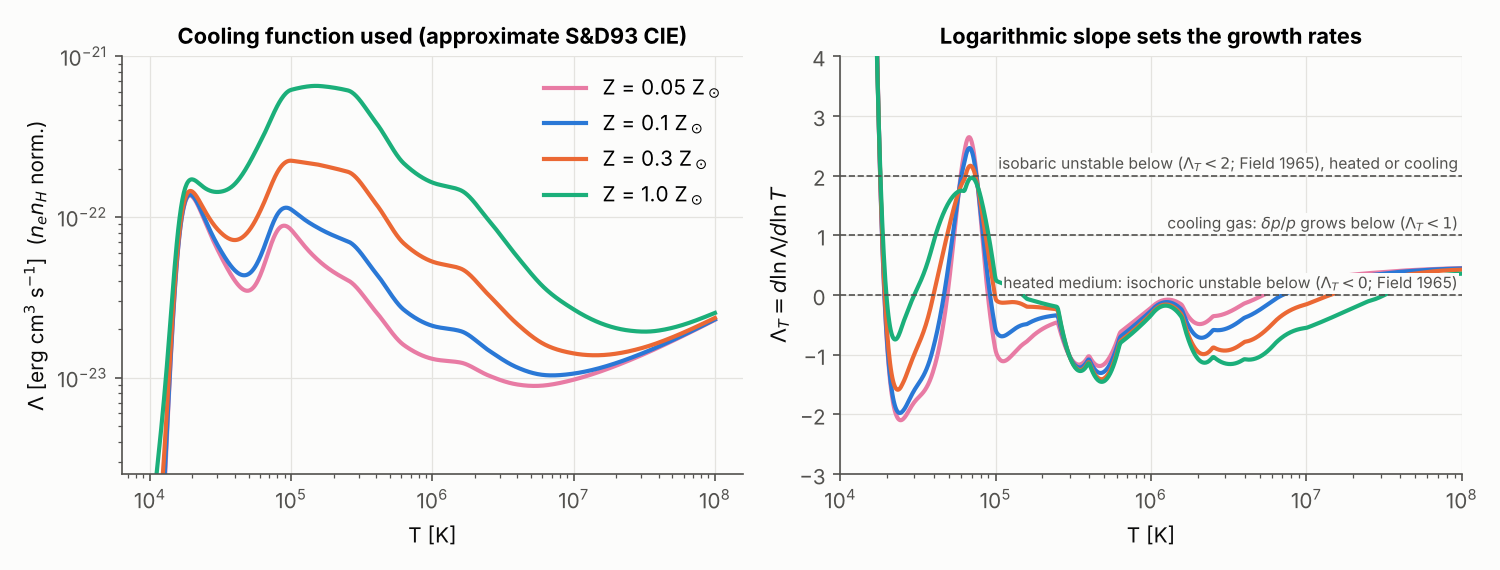
\includegraphics[width=\textwidth]{fig1_cooling_function.png}
\caption{Original approximate collisional-equilibrium cooling function (left)
and its logarithmic slope $\LT=d\ln\Lambda/d\ln T$ (right) for four
metallicities. Horizontal lines mark the stability thresholds discussed in
Section~\ref{sec:linear}.}
\label{fig:cooling}
\end{figure}

%======================================================================
\section{Linear theory on a cooling background}
\label{sec:linear}
%======================================================================

\subsection{Equations}
We follow one Fourier mode in the Lagrangian mass coordinate $m$ on a uniform
background that cools. Write
$\drho = s(t)\cos(k_m m)$, $\delta p/p = q(t)\cos(k_m m)$ and
$\delta v = w(t)\sin(k_m m)$, with physical wavenumber $k=k_m\rho_0$. Let
$D=d\ln\rho_0/dt$, let $L(\rho,T)$ be the net radiative loss per unit volume,
$r=(\gamma-1)L/p_0$, and $L_\rho=\partial L/\partial\ln\rho$,
$L_T=\partial L/\partial\ln T$, $L_Z=\partial L/\partial\ln Z$. Then
\begin{align}
\frac{ds}{dt} &= sD - kw, \label{eq:s}\\
\frac{dw}{dt} &= k\,\frac{p_0}{\rho_0}\,q, \label{eq:w}\\
\frac{dq}{dt} &= qr + \gamma sD - \gamma kw
  - \frac{\gamma-1}{p_0}\left[L_\rho s + L_T(q-s)\right]
  - \frac{\gamma-1}{p_0}L_Z\zeta, \label{eq:q}
\end{align}
where $\zeta=\delta Z/Z$ is a metallicity perturbation, constant on each fluid
element. The \emph{infinite medium} has $D=0$ and cools at constant density. A
\emph{small cloud} ($L\ll\cstc$) held at the constant pressure of the hot gas has
$D=r/\gamma$, so it is compressed as it cools and $k$ grows with $\rho_0$. For
collisional cooling $L_\rho=2L$ and $L_T=\LT L$. The background equations are
integrated together with
Eqs.~(\ref{eq:s})--(\ref{eq:q}), using the same cooling tables and interpolation
as gPLUTO.

\subsection{Limits}
\paragraph{Short wavelength (isobaric).} Pressure equalizes quickly ($q\to0$)
and
\begin{equation}
\frac{ds}{dt}=\frac{2-\LT}{\gamma\,\tcool(t)}\,s,\qquad
\tcool(t)\equiv\frac{p_0}{(\gamma-1)L}.
\label{eq:isobaric}
\end{equation}
This is the same instantaneous rate as the isobaric mode of \citet{das21}.
Integrating it along the cooling background gives a closed form: a short-wavelength
perturbation is a \emph{time shift} of the cooling history (the denser parcel
reaches each temperature a little earlier), with
\begin{equation}
\frac{s(T)}{s_0}=\left[\left(\frac{T_0}{T}\right)^2\frac{\Lambda(T)}{\Lambda(T_0)}\right]^{\beta},
\qquad \beta=\begin{cases}1 & \text{small cloud (isobaric background)},\\
1/\gamma & \text{infinite medium (isochoric background)}.\end{cases}
\label{eq:timeshift}
\end{equation}

\paragraph{Long wavelength (isochoric).} The density is frozen ($s$ constant)
while
\begin{equation}
\frac{dq}{dt}=\frac{(1-\LT)\,q-(2-\LT)\,s}{\tcool}.
\label{eq:isochoric}
\end{equation}
The temperature and pressure perturbation is driven by the frozen density
perturbation, and grows on its own wherever $\LT<1$. In the heated medium of
\citet{das21} the corresponding condition is $\LT<0$.

\subsection{Why the amplification is much larger than in a heated medium}
\label{sec:whyheated}
In the heated medium of \citet{das21} the background is steady: heating balances
cooling, $\tcool$ stays at its initial value $t_{\rm cool,0}$, and a short-wavelength
mode grows exponentially at the \emph{constant} rate
$\sigma_0=(2-\LT)/(\gamma t_{\rm cool,0})$, i.e.\ $G=\exp(\sigma_0 t)$.

In cooling gas the instantaneous rate is given by the same formula,
Eq.~(\ref{eq:isobaric}), but $\tcool$ is evaluated at the \emph{current}
temperature, and it collapses as the gas cools. At constant density
$\tcool\propto T/\Lambda(T)$; at constant pressure $\propto T^2/\Lambda(T)$.
Table~\ref{tab:sigma} follows an infinite medium with $n=10^{-2}$\,cm$^{-3}$,
$Z=0.3$, starting at $10^6$\,K.

\begin{table}[H]
\centering
\small
\caption{Cooling time and instantaneous isobaric growth rate along the cooling
history of an infinite medium ($n=10^{-2}$\,cm$^{-3}$, $Z=0.3$, original
cooling). The last column is the rate in units of the initial rate
$\sigma_0=0.042$\,Myr$^{-1}$.}
\label{tab:sigma}
\begin{tabular}{rrrrr}
\toprule
$T$ [K] & $\tcool$ [Myr] & $\LT$ & $\sigma=(2-\LT)/(\gamma\tcool)$ [Myr$^{-1}$] & $\sigma/\sigma_0$ \\
\midrule
$10^6$            & 33.5  & $-0.32$ & 0.042 & 1 \\
$5\times10^5$     & 9.9   & $-1.40$ & 0.21  & 5 \\
$3\times10^5$     & 3.1   & $-1.03$ & 0.58  & 14 \\
$10^5$            & 0.79  & $-0.06$ & 1.6   & 38 \\
$3\times10^4$     & 0.63  & $-0.99$ & 2.9   & 69 \\
$2\times10^4$     & 0.25  & $-0.59$ & 6.3   & 150 \\
\bottomrule
\end{tabular}
\end{table}

The number of e-folds is $N=\int\sigma\,dt$. Over the 20\,Myr the gas takes to
cool from $10^6$ to $1.5\times10^4$\,K:
\begin{itemize}
\item the heated medium accumulates $\sigma_0\times20\,{\rm Myr}=0.84$ e-folds,
  a factor 2.3;
\item the cooling gas accumulates $N=4.9$ e-folds, a factor $\approx130$. Of
  these, 2.1 come from the first 17\,Myr ($10^6$--$3\times10^5$\,K), and 2.7 from
  the last 3\,Myr ($3\times10^5$--$2\times10^4$\,K). This equals the time-shift
  result, Eq.~(\ref{eq:timeshift}) with $\beta=1/\gamma$, evaluated at
  $1.5\times10^4$\,K.
\end{itemize}
So the cooling gas amplifies far more \emph{in the same elapsed time} because it
sweeps through temperatures where the cooling time, and hence the growth time,
is up to a hundred times shorter. Two caveats keep the comparison fair. First,
the heated medium is not capped: it keeps growing and reaches a factor of 100
after $\approx110$\,Myr ($3.3\,t_{\rm cool,0}$), whereas the cooling gas cannot
amplify beyond what Eq.~(\ref{eq:timeshift}) allows, about $10^2$ in an infinite
medium and $\sim3\times10^3$ in a small cloud from $10^6$\,K. Second, this is the
short-wavelength limit; at $\lambda\gtrsim\cstc$ both cases grow much less.

%======================================================================
\section{Results}
\label{sec:results}
%======================================================================

\subsection{Validation}
Periodic gPLUTO runs with $A=10^{-4}$ match the linear theory to 3--4 significant
figures through the whole cooling history, for $\lambda/(\cstc)=0.1$, 1 and 10,
with the original cooling (Figure~\ref{fig:validation}) and with the UV
background (Figure~\ref{fig:validationuvb}). The five seed types of
Section~\ref{sec:seeds} match equally well (Figure~\ref{fig:perthist}).

\begin{figure}[H]
\centering
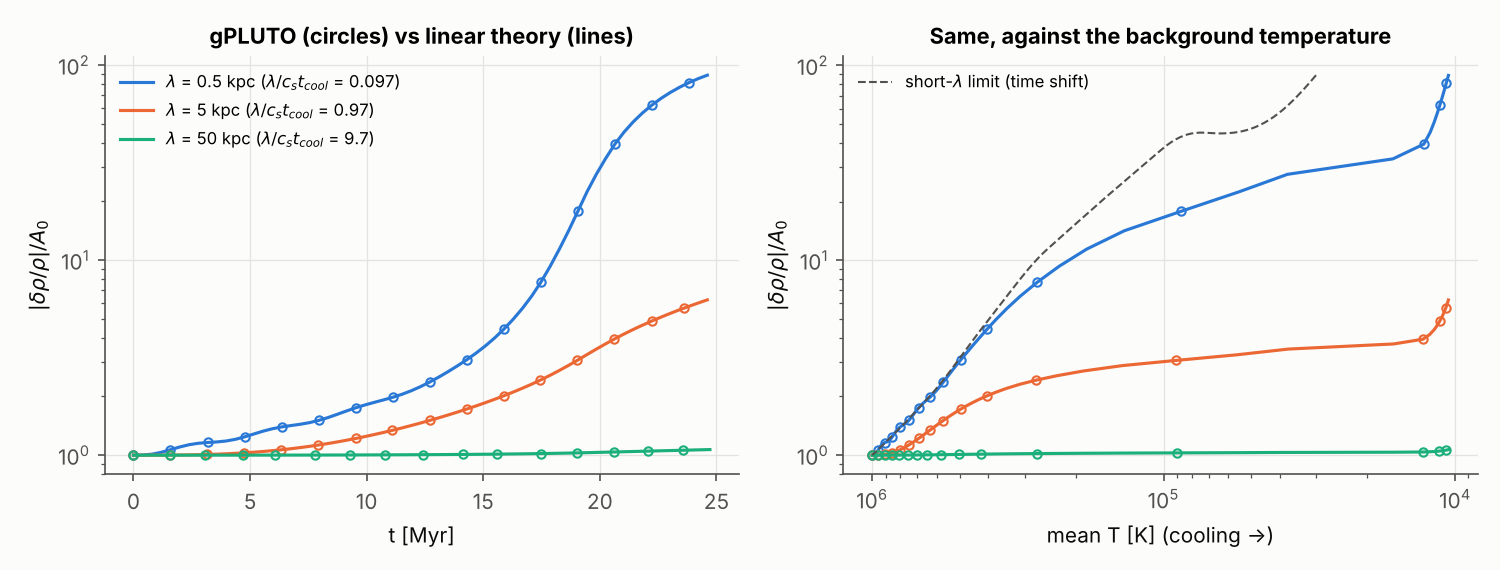
\includegraphics[width=\textwidth]{fig2_validation.png}
\caption{Infinite medium, $n=10^{-2}$\,cm$^{-3}$, $Z=0.3$, $T_0=10^6$\,K,
original cooling. Circles: gPLUTO; lines: linear theory. Left: mode amplitude
against time. Right: against the background temperature; the dashed curve is
the short-wavelength time-shift limit, Eq.~(\ref{eq:timeshift}).}
\label{fig:validation}
\end{figure}

\subsection{Growth versus $\lambda/(\cstc)$}
\label{sec:growthx}
Table~\ref{tab:inf} and Figure~\ref{fig:linear} give the amplification of an
infinite medium. In a small cloud held at constant pressure, the compression adds
a large factor: $\sim10^3$ while cooling at $x\lesssim0.1$ and
$\sim3$--$4\times10^3$ by $3\,\tcool$. Metallicity enters mostly through $\cstc$; at
fixed $x$, $Z=0.05$ and $Z=1$ differ by $\lesssim30\%$. Starting cooler leaves
less of the cooling curve to traverse: from $2.5\times10^5$\,K the
infinite-medium amplification is $\lesssim25$ (Figure~\ref{fig:linearT0}).

\begin{table}[H]
\centering
\small
\caption{Linear-theory amplification of an infinite medium starting at
$10^6$\,K ($Z=0.3$, original cooling). The simulations agree
(Figure~\ref{fig:infsims}).}
\label{tab:inf}
\begin{tabular}{lrrrrrr}
\toprule
$x=\lambda/(\cstc)$ & 0.03 & 0.1 & 0.3 & 1 & 3 & 10 \\
\midrule
growth while cooling & 71 & 33 & 11 & 3.6 & 1.3 & 1.03 \\
growth by $3\,\tcool$ & 124 & 103 & 66 & 24 & 4 & 1.3 \\
\bottomrule
\end{tabular}
\end{table}

\begin{figure}[H]
\centering
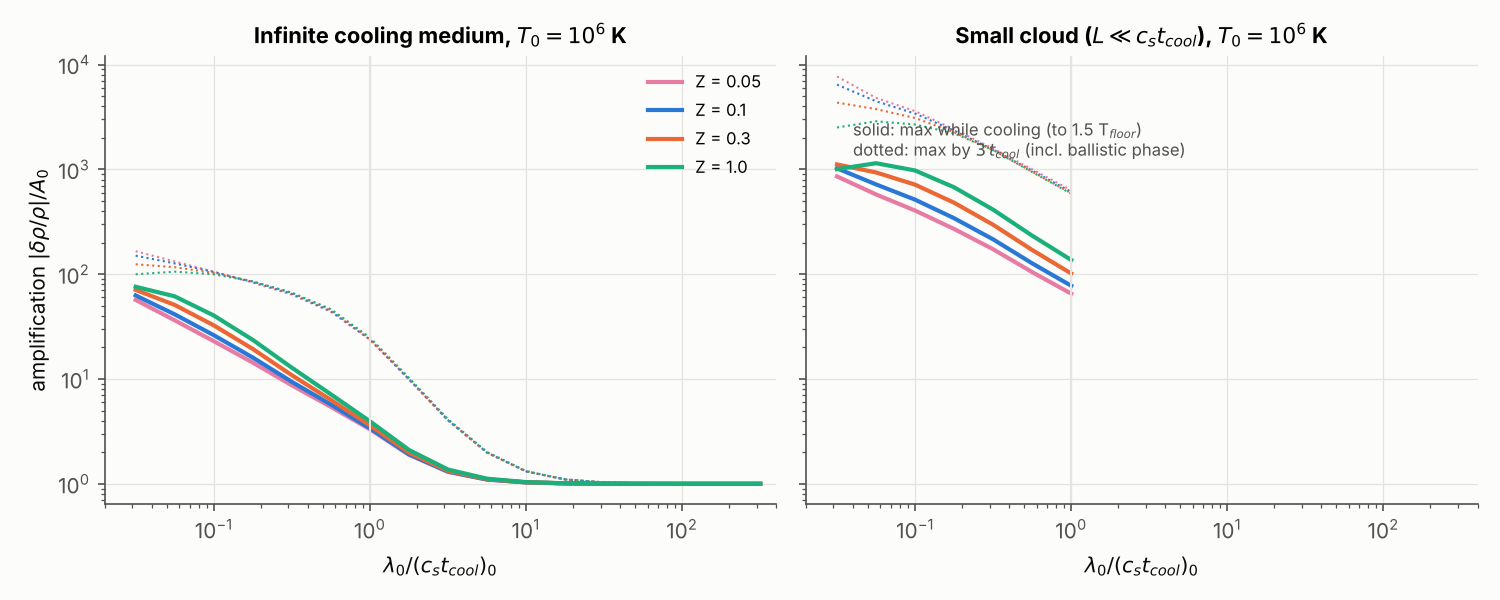
\includegraphics[width=\textwidth]{fig3_linear_amplification.png}
\caption{Linear-theory amplification against $\lambda_0/(\cstc)_0$ for four
metallicities, $T_0=10^6$\,K. Left: infinite medium. Right: small cloud at
constant pressure (shown only for $\lambda<\cstc$, where it applies). Solid: maximum
while cooling; dotted: maximum by $3\,\tcool$. Dashed grey: growth of the same
mode in the heated medium of \citet{das21} over the same elapsed time
(Section~\ref{sec:whyheated}).}
\label{fig:linear}
\end{figure}

\begin{figure}[H]
\centering
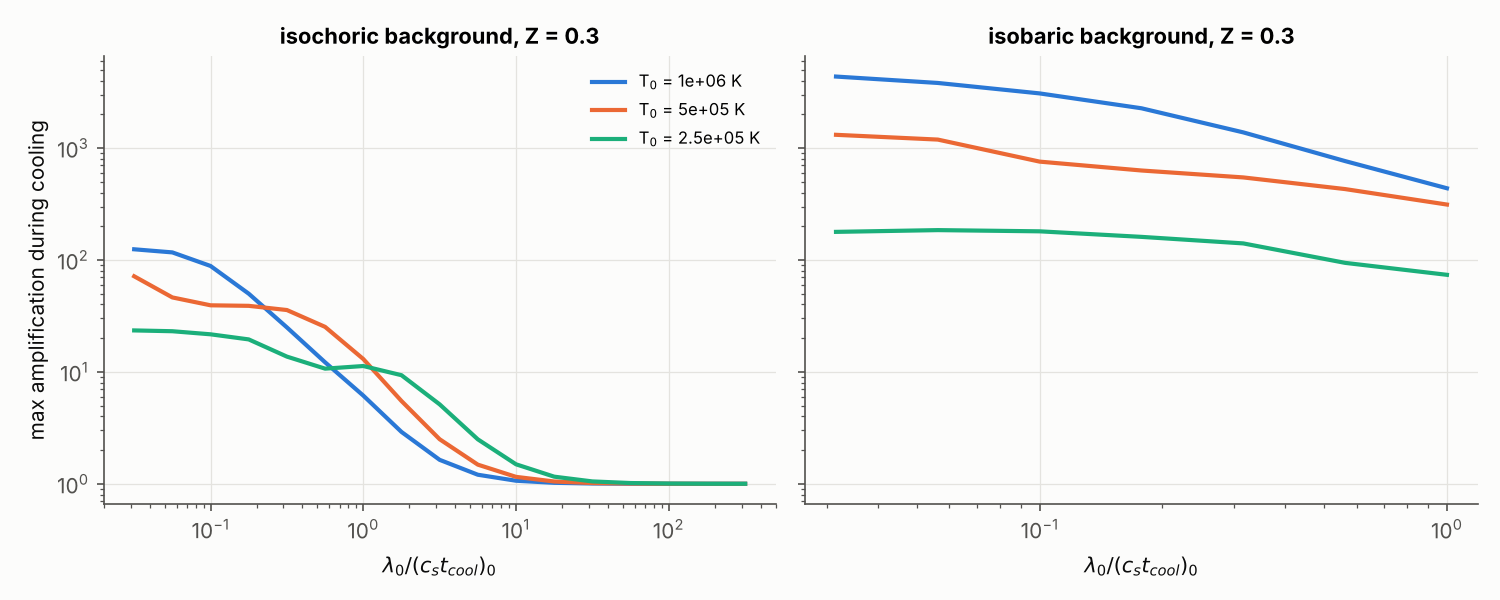
\includegraphics[width=\textwidth]{fig3b_linear_amplification_T0.png}
\caption{As Figure~\ref{fig:linear} (growth while cooling, $Z=0.3$) for three
initial temperatures.}
\label{fig:linearT0}
\end{figure}

Figure~\ref{fig:minamp} turns this into the smallest seed that reaches
$\drho\sim1$ by $3\,\tcool$. In an infinite medium or a large cloud it is about
1\% for $x\lesssim0.3$, 4\% at $x=1$ and 25\% at $x\approx3$; for $x\gtrsim10$ no
seed below order unity gets there. In a small isobaric cloud it is
$2\times10^{-4}$ to $2\times10^{-3}$.

\begin{figure}[H]
\centering
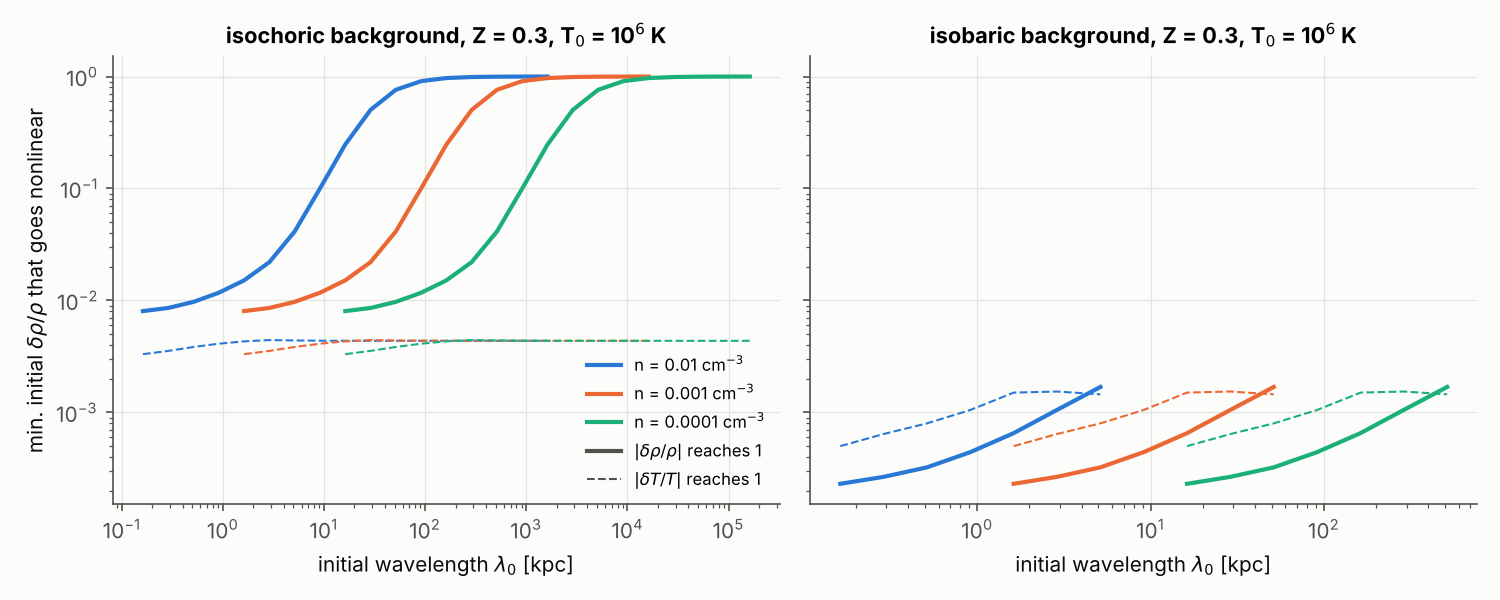
\includegraphics[width=\textwidth]{fig4_min_amplitude_nonlinear.png}
\caption{Smallest initial $\drho$ that reaches order unity by $3\,\tcool$
(linear theory), against the initial wavelength in kpc, for three densities.
With collisional cooling the curves are the same function of
$\lambda/(\cstc)$, shifted because $\cstc\propto1/n$.}
\label{fig:minamp}
\end{figure}

The 63 infinite-medium simulations (Figure~\ref{fig:infsims}) follow the linear
theory for $A\le10^{-2}$. For $A=0.1$ the growth saturates near 15 ($\drho\approx1.5$)
and the gas condenses into clumps 30--45 times denser than the mean for $x\lesssim1$.

\begin{figure}[H]
\centering
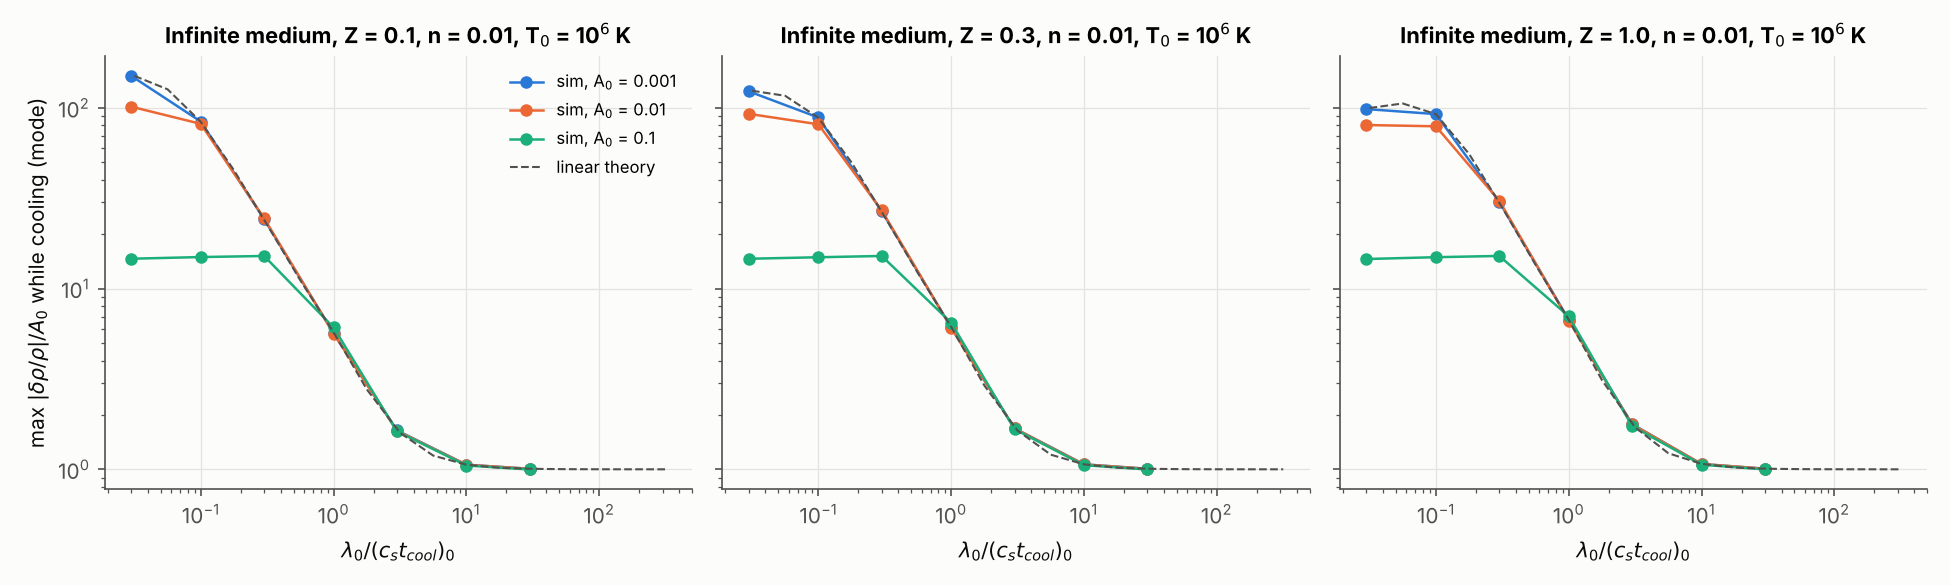
\includegraphics[width=\textwidth]{fig5_infinite_sims.png}
\caption{Infinite-medium simulations (points) for three seed amplitudes and three
metallicities, against linear theory (dashed). The $A=0.1$ runs saturate in the
nonlinear regime.}
\label{fig:infsims}
\end{figure}

\subsection{Clouds}
\label{sec:clouds}
Figure~\ref{fig:clouds} collects all 62 cloud runs. Clouds with
$L\gtrsim1.5\,\cstc$ lie on the infinite-medium curve: the interior of a large
cloud behaves like an infinite medium. Smaller clouds lie between the
infinite-medium and small-cloud limits. Typical values for $\chi=2$ are in
Table~\ref{tab:clouds}.

\begin{table}[H]
\centering
\small
\caption{Growth of the seeded mode in cloud runs with $\chi=2$ and $L\ge1.5\,\cstc$
(medians in bins of $x$).}
\label{tab:clouds}
\begin{tabular}{lrrrrr}
\toprule
$x=\lambda/(\cstc)$ & $\sim0.2$ & $\sim1$ & $\sim2$ & $\sim5$ & $\ge10$ \\
\midrule
growth while cooling & 18 & 4 & 1.9 & 1.2 & 1.0 \\
growth by $2.5\,\tcool$ & 32 & 15 & 5.8 & 2.2 & 1.06 \\
\bottomrule
\end{tabular}
\end{table}

\begin{figure}[H]
\centering
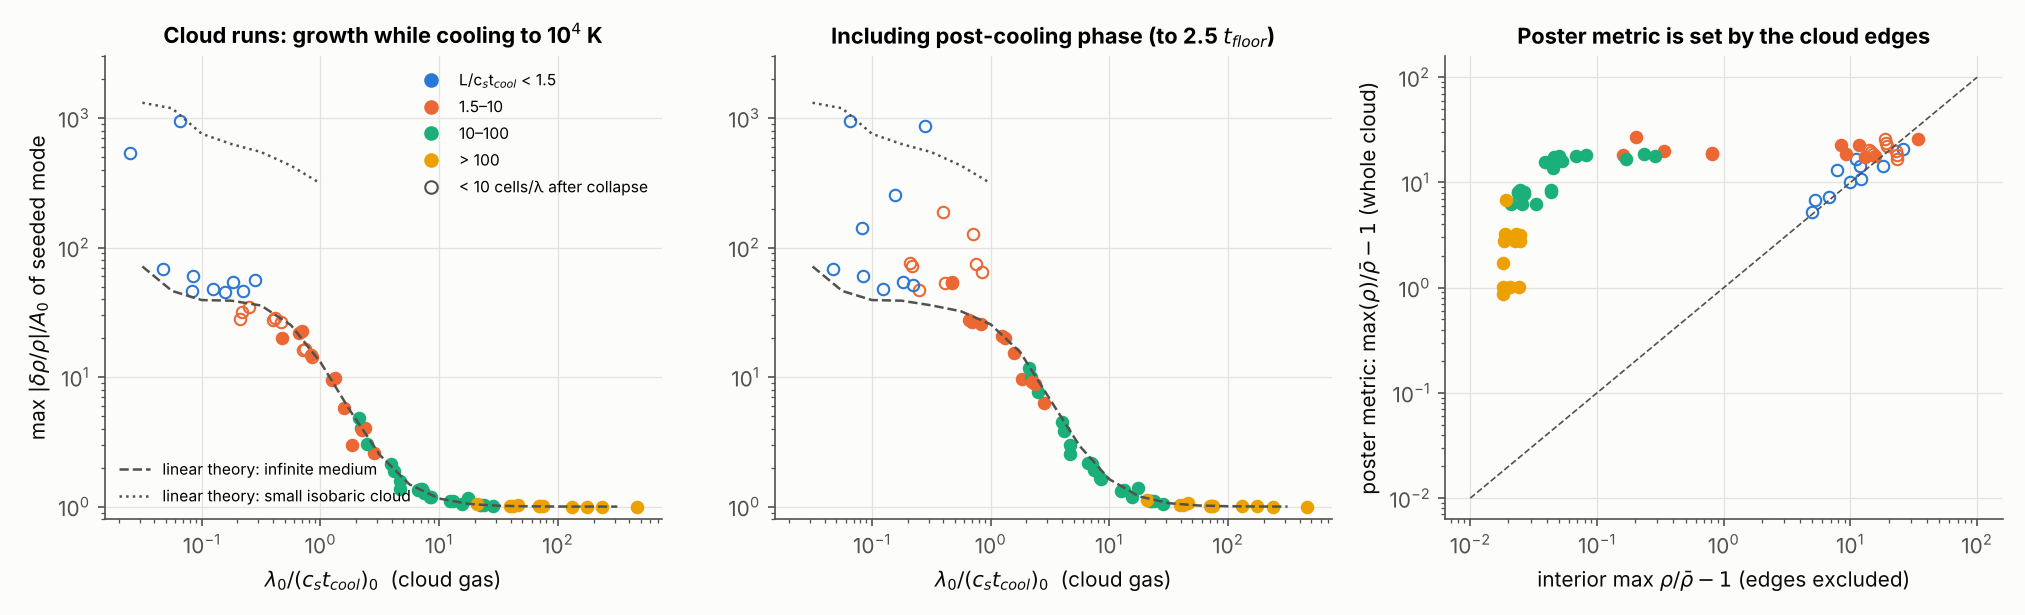
\includegraphics[width=\textwidth]{fig6_cloud_sweep.png}
\caption{All 62 cloud runs (original cooling). \textbf{Every run has 2048 cells;
the symbols do not encode the cell count.} Colour encodes the cloud size in units of
the cooling length, $L/(\cstc)$, in four bins. Filled symbols are
well resolved; \textbf{open symbols mark runs in which the cloud was compressed so
much that, after the compression, the seeded wavelength spans fewer than 10
cells}, so their late-time values are unreliable (Section~\ref{sec:resolution}).
Left: growth while cooling; middle: by $2.5\,\tcool$; dashed and dotted lines are
the infinite-medium and small-cloud linear theory. Right: a maximum of
$\rho/\bar\rho-1$ over the whole cloud (including the edges) against the interior
maximum. The whole-cloud value is dominated by the compressed edges, which is why
the interior should be used, as in the student's analysis.}
\label{fig:clouds}
\end{figure}

\begin{figure}[H]
\centering
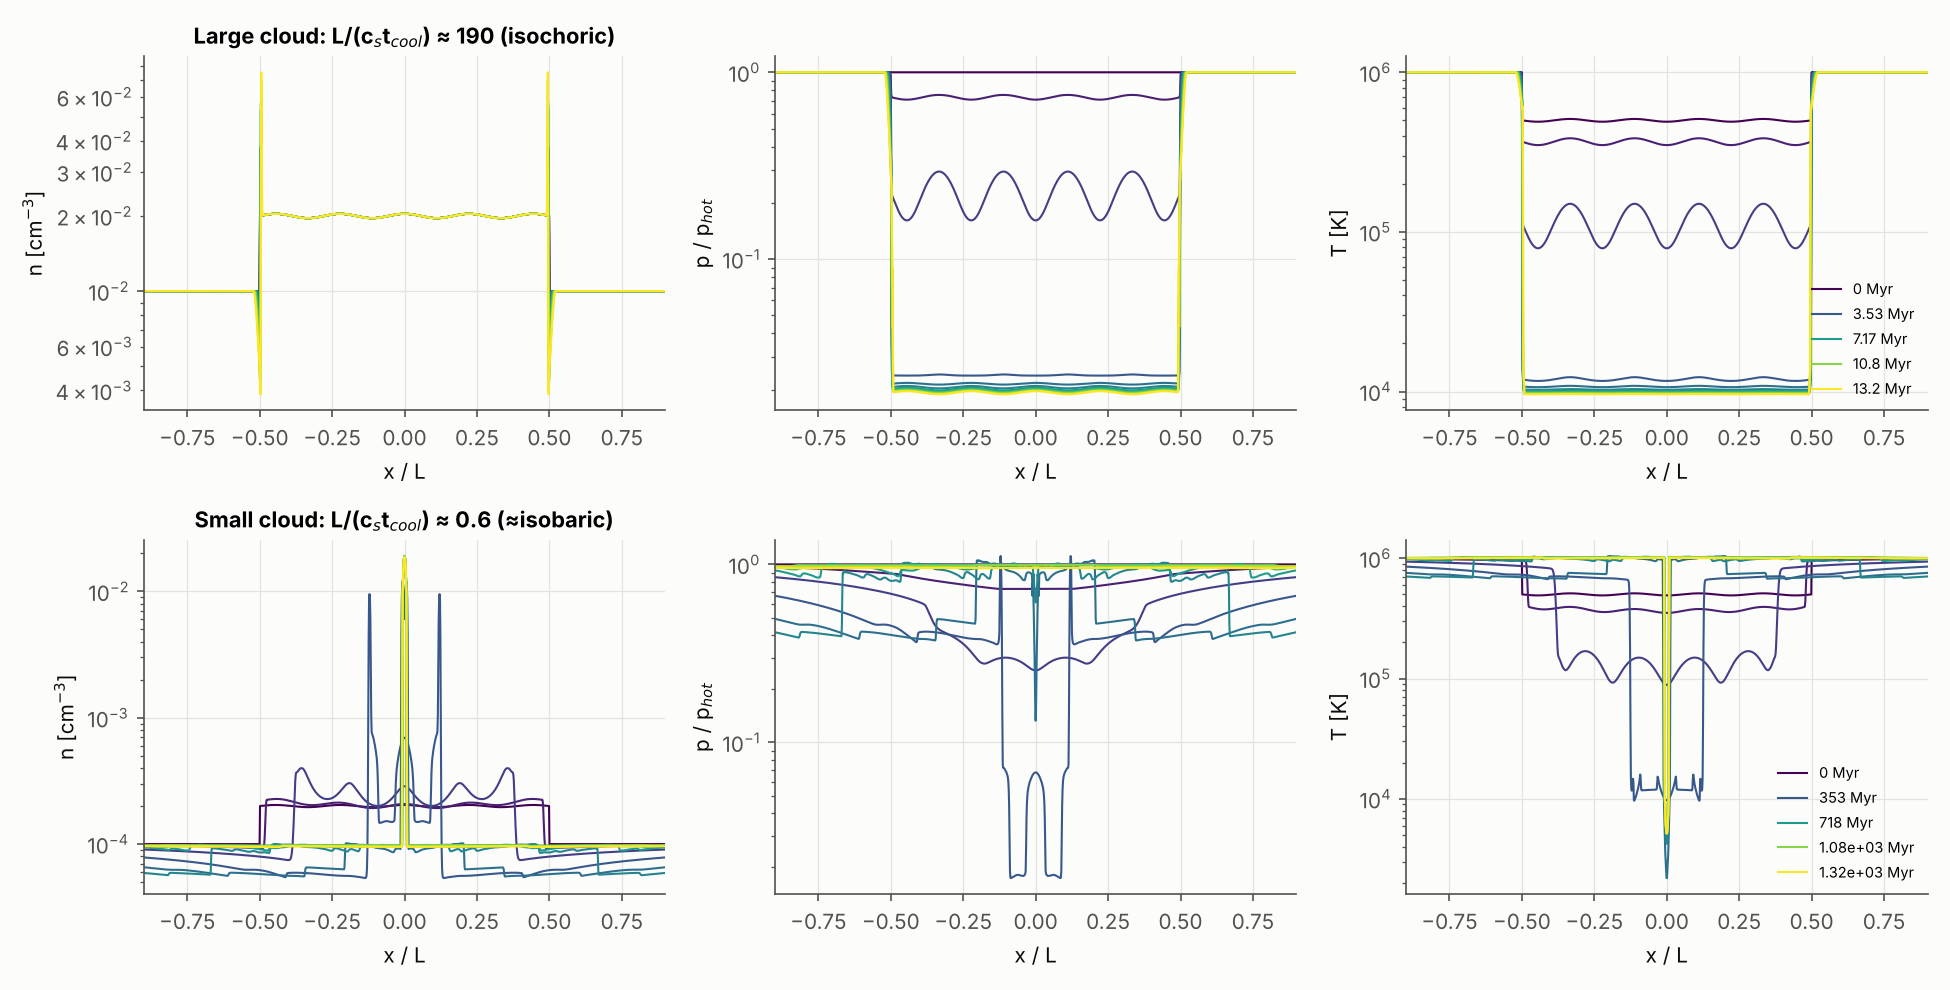
\includegraphics[width=\textwidth]{fig7_profiles.png}
\caption{Density, pressure and temperature profiles at several times. Top: a large
cloud ($L\approx190\,\cstc$); it cools at constant density, its pressure drops
by a factor 50, and the seeded mode does not grow while the edges are
compressed. Bottom: a cloud with $L\approx0.6\,\cstc$; it is compressed as it
cools, the perturbation goes nonlinear around $10^5$\,K, and the cold gas
collapses to a thin slab.}
\label{fig:profiles}
\end{figure}

\subsection{Clouds with no initial contrast ($\chi=1$)}
\label{sec:chi1}
The simplest version of the setup has no density or temperature jump at all: the
``cloud'' is background gas at $10^6$\,K in which cooling is switched on, with
the seed on top. The model then depends only on $L/(\cstc)$, $\lambda/(\cstc)$,
$Z$ and the seed, and the periodic infinite medium is its $L\to\infty$ limit.
Thirty-six runs ($Z=0.3$; $n_{\rm bg}=10^{-4},10^{-3},10^{-2}$; $L=30$ and 100\,kpc;
2.5, 4.5 and 8.5 wavelengths per cloud; original cooling and UV background) span
$L/(\cstc)=0.05$--20. Resolved clouds lie on the infinite-medium curves while
cooling and afterwards (Figure~\ref{fig:chi1}). Small clouds ($L\lesssim\cstc$)
collapse by $\sim100$ in density to slabs a few cells wide, and their late-time
values are not reliable.

Figure~\ref{fig:chi1prof} shows a striking case. At $L\approx1.5\,\cstc$ with the
UV background, the cloud breaks into cold dense sheets at the crests of the seed,
while the gas between them expands, its cooling time lengthens, and it stays at
$\sim6\times10^5$\,K through $3\,\tcool$: a two-phase structure grown from a 2\%
seed.

\begin{figure}[H]
\centering
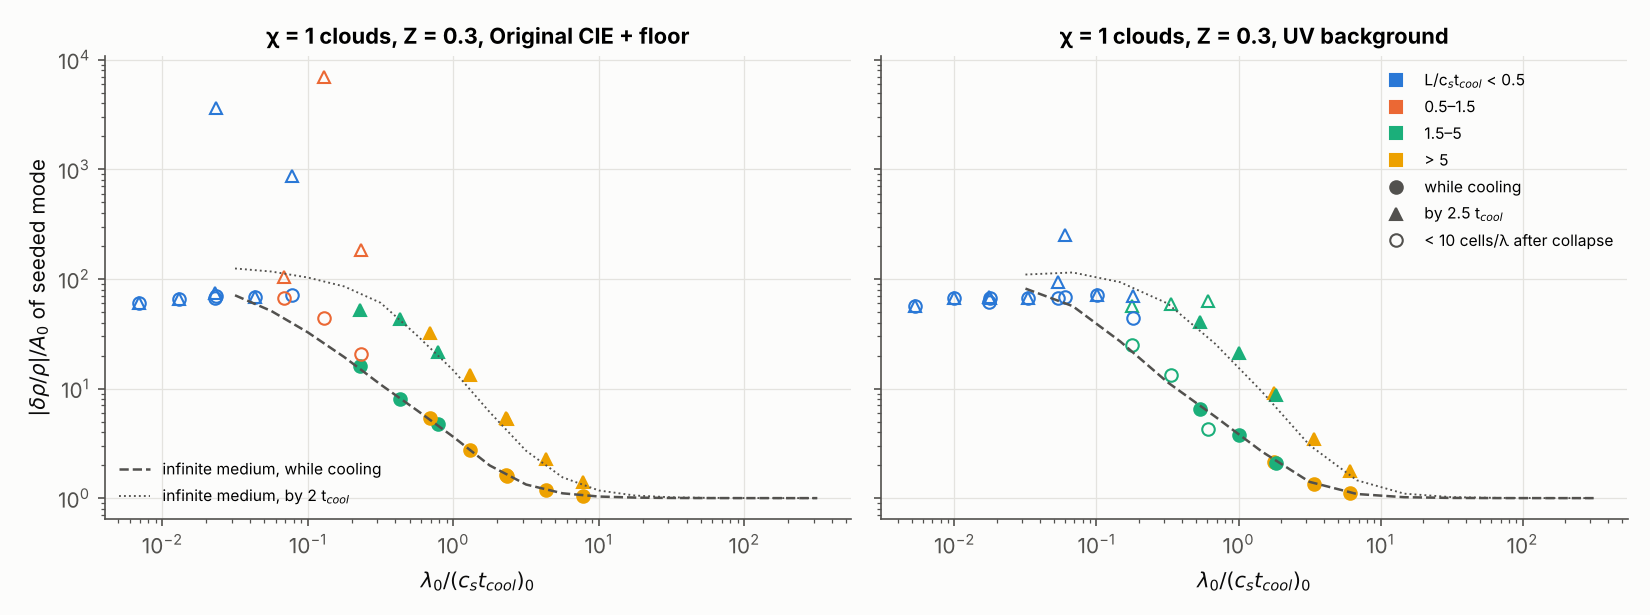
\includegraphics[width=\textwidth]{fig22_chi1_clouds.png}
\caption{$\chi=1$ clouds: growth of the seeded mode while cooling (circles) and by
$2.5\,\tcool$ (triangles), coloured by $L/(\cstc)$, with the infinite-medium
linear theory. All runs have 2048 cells; open symbols mark runs whose seeded
wavelength spans fewer than 10 cells after the cloud's collapse.}
\label{fig:chi1}
\end{figure}

\begin{figure}[H]
\centering
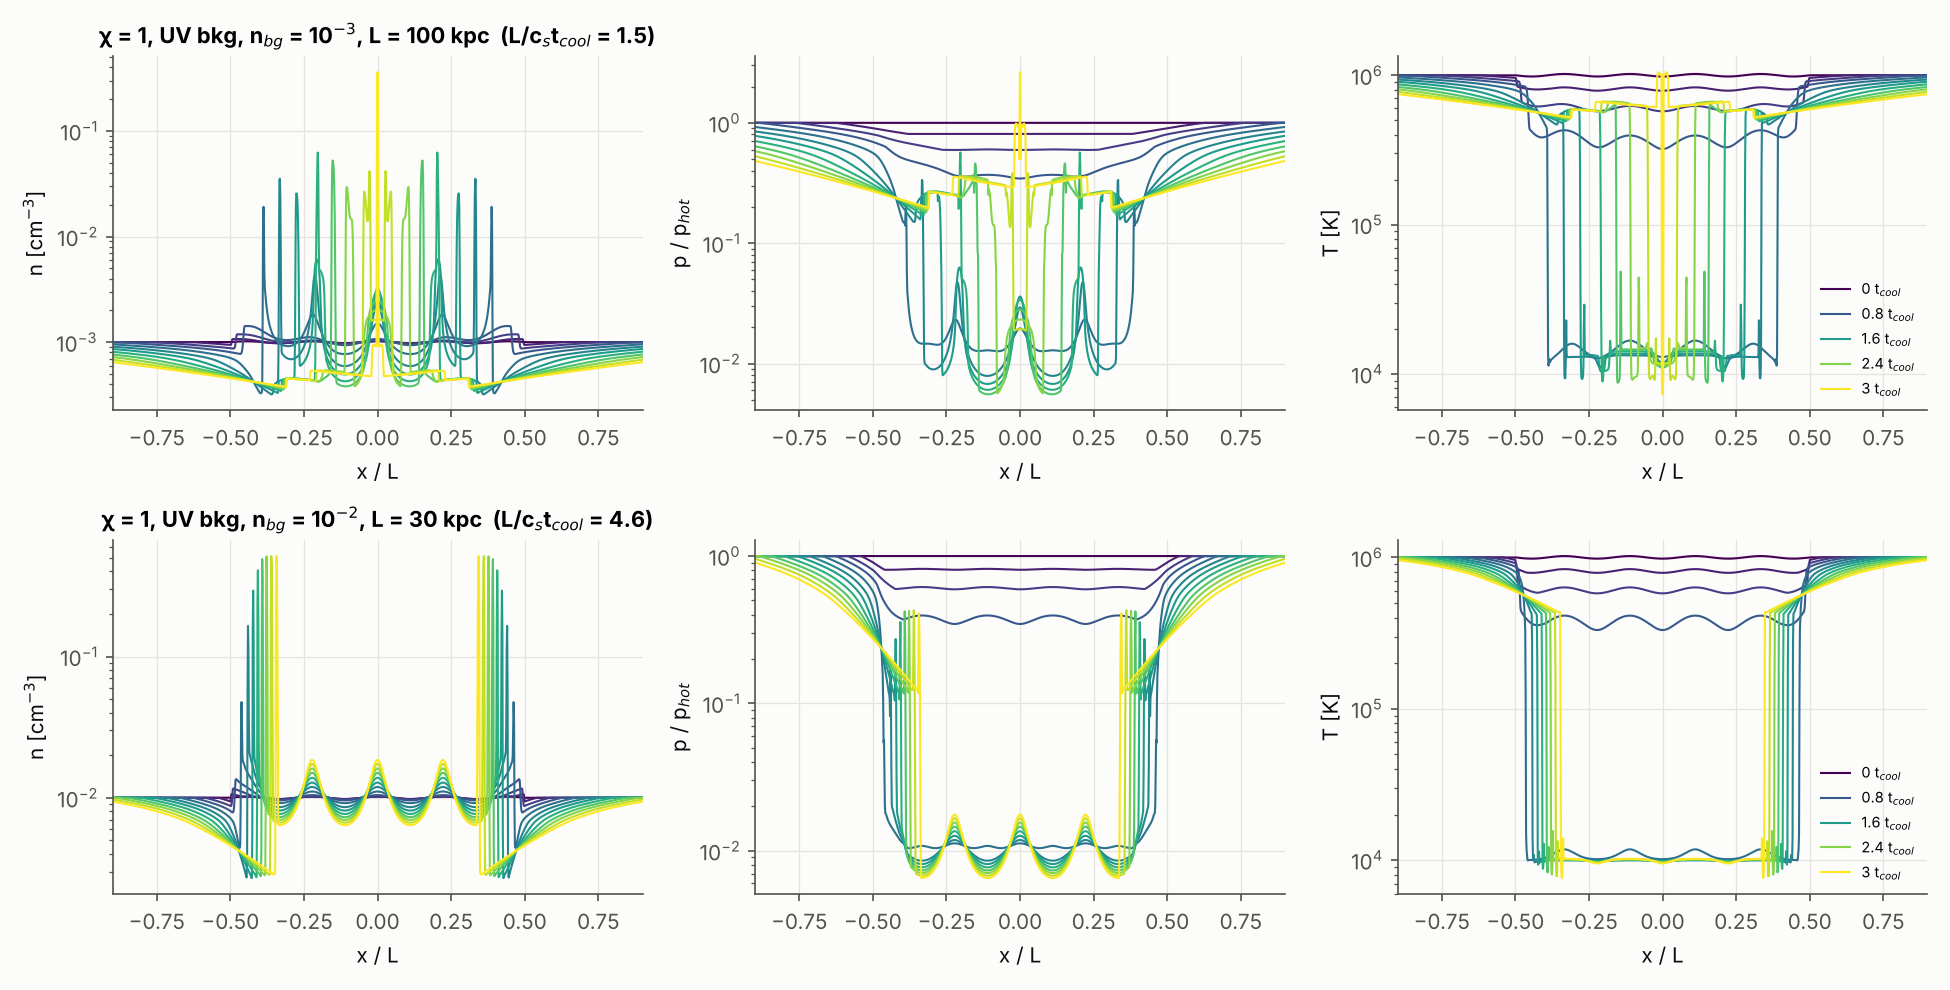
\includegraphics[width=\textwidth]{fig23_chi1_profiles.png}
\caption{Profiles of two $\chi=1$ clouds with the UV background. Top
($L\approx1.5\,\cstc$): the cloud splits into cold sheets separated by hot,
dilute gas. Bottom ($L\approx4.6\,\cstc$): the interior cools nearly uniformly and
the seeded mode grows slowly.}
\label{fig:chi1prof}
\end{figure}

\paragraph{The cooling switch and numerical mixing.}
The tracer that switches cooling on is advected with the gas, so the cooling
region moves inward with the cloud as it contracts and hot gas flowing in behind
it does not cool. The only non-Lagrangian part is numerical diffusion at the
cloud edge: cells there contain a mix of cloud and background gas and cool
partially. The edge stays sharp (4--8 mixed cells), but once a cloud has
collapsed, hot gas flowing onto the cold slab is mixed into it numerically and
cools. Table~\ref{tab:mask} tests this on a collapsing $\chi=1$ cloud.

\begin{table}[H]
\centering
\small
\caption{Hot background gas that ends up cold, relative to the initial cloud mass,
for a $\chi=1$ cloud with $L\approx0.5\,\cstc$ (UV background, $n_{\rm bg}=10^{-3}$).
``Proportional'': cooling multiplied by the tracer. ``Sharp'': cooling only where
the tracer exceeds 0.5.}
\label{tab:mask}
\begin{tabular}{lccc}
\toprule
switch, cells & growth while cooling & at $1.6\,\tcool$ & at $2.4\,\tcool$ \\
\midrule
proportional, 2048 & 71.5 & 18\% & 25\% \\
sharp, 2048        & 71.6 & 16\% & 23\% \\
proportional, 8192 & 71.4 & 10\% & 14\% \\
\bottomrule
\end{tabular}
\end{table}

The growth while cooling is unaffected. The leakage appears only after collapse;
a sharp switch barely helps, and it decreases only slowly with resolution. Across
the $\chi=1$ set it is 2--3\% for large clouds, 7--11\% for $L\approx5\,\cstc$ and
up to $\sim40\%$ for clouds that collapse to a few cells. (For $\chi=2$ clouds it is
0.3--9\%.) This is a limitation of any fixed-grid code; a switch based on a
density threshold would be worse, because compressed hot gas crosses the
threshold. In 1D the clean solution is a Lagrangian (mass-coordinate) code, in
which the cooling switch is exactly attached to the gas and a collapsing cloud
keeps its resolution automatically.

\subsection{The isochoric regime}
\label{sec:isochoric}
For $\lambda\gg\cstc$ each parcel cools at its own fixed density. The cooling rate
per particle is $\propto n\Lambda(T)$, so denser parcels run ahead in
temperature: $\delta T/T=\delta p/p$ grows 12--50 times during cooling (to
0.24--1.0 from $\drho=0.02$), independent of $\lambda$. That pressure pattern
pushes gas from the hotter, underdense parcels into the colder ones. During the
cooling time the gas moves only $\sim(\cstc/\lambda)^2$ of a wavelength, but the
velocity persists after cooling, so the density keeps growing roughly linearly in
time. All 37 cloud runs with $\lambda=2$--$460\,\cstc$ and $L\ge1.5\,\cstc$ follow
\begin{equation}
G-1\approx25\left(\frac{\cstc}{\lambda}\right)^2\quad\text{by }2.5\,\tcool
\label{eq:isoscaling}
\end{equation}
(10--90\% range of the prefactor: 21--29; Figure~\ref{fig:isochoric}). This is
the scaling expected for a pressure impulse of order $\delta T/T$ acting for
$\sim\tcool$ across a wavelength. The prefactor keeps growing; the convergence
completes on the sound-crossing time of $\lambda$ in the cold gas, $\approx7x\,\tcool$
for gas starting at $5\times10^5$\,K, well beyond our runs and the poster's. If
$\delta T/T$ reaches order unity during cooling, parts of the cloud reach the floor
while their neighbours are still hot and are crushed; this is the isochoric
fragmentation picture of \citet{mccourt18}.

\begin{figure}[H]
\centering
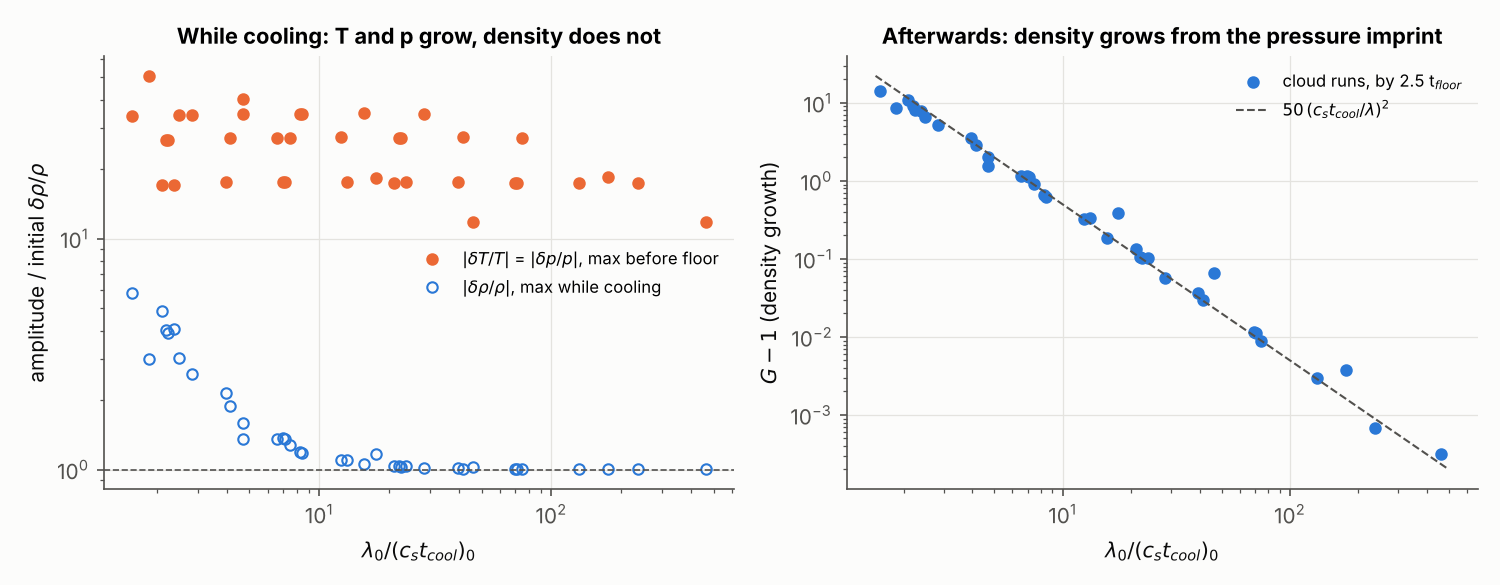
\includegraphics[width=\textwidth]{fig11_isochoric_regime.png}
\caption{Cloud runs with $\lambda\ge1.5\,\cstc$ and $L\ge1.5\,\cstc$. Left: during
cooling the temperature/pressure perturbation grows (filled) while the density
perturbation does not (open). Right: density growth by $2.5\,\tcool$ follows
Eq.~(\ref{eq:isoscaling}) over two decades in $\lambda$.}
\label{fig:isochoric}
\end{figure}

\subsection{Seed amplitude and resolution}
\label{sec:resolution}
For a cloud with $L=50$\,kpc, $\chi=2$, $Z=0.3$ (Figure~\ref{fig:amplitude}):
\begin{itemize}
\item $n_{\rm bg}=10^{-2}$ ($L\approx90\,\cstc$): nothing grows for any $A\le0.3$;
\item $n_{\rm bg}=10^{-3}$ ($L\approx9\,\cstc$): every seed grows the same way,
  $\times2$ while cooling and $\times6.5$ by $2.5\,\tcool$, linear until
  $A\approx0.1$; $A=0.3$ goes nonlinear after $\sim2.5\,\tcool$;
\item $n_{\rm bg}=10^{-4}$ ($L\approx0.9\,\cstc$): $\sim50\times$ growth while
  cooling and much more during the collapse that follows. Even $A=10^{-3}$ reaches
  an interior contrast of $\sim15$, which then smooths out to $\lesssim0.1$.
\end{itemize}

\begin{figure}[H]
\centering
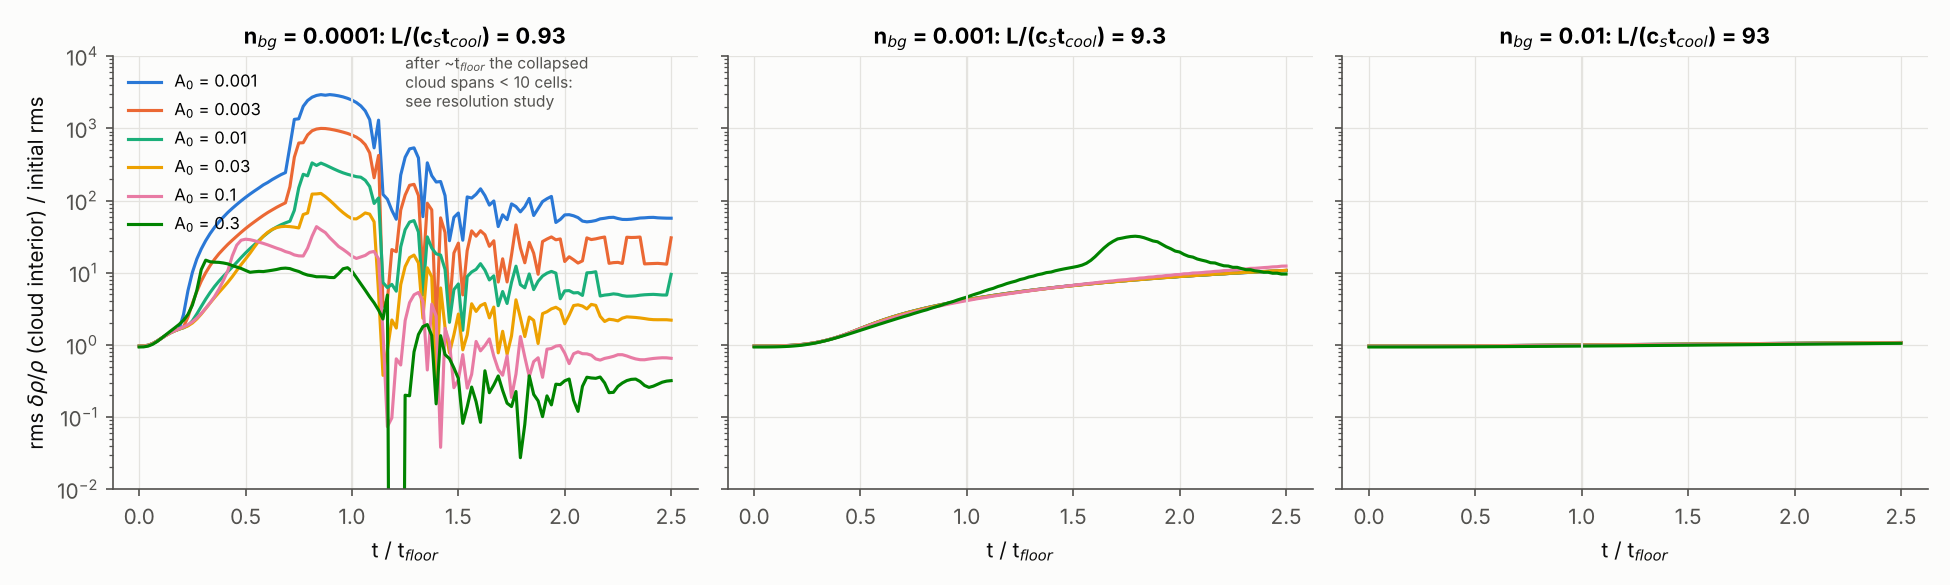
\includegraphics[width=\textwidth]{fig8_amplitude_scan.png}
\caption{Interior rms $\drho$ (normalized to its initial value) for six seed
amplitudes, at three background densities. Original cooling.}
\label{fig:amplitude}
\end{figure}

The small cloud is compressed 200--350 times in density and is the hardest case
to resolve (Figure~\ref{fig:resolution}). Comparing 2048, 4096 and 16384 cells,
the growth while cooling is converged (52, 52, 51 for $A=10^{-3}$); the peak
contrast is converged for small seeds (14, 18, 19) but not for $A=0.1$ (28, 47,
75; a lower limit); the late-time smoothing appears at every resolution.

\begin{figure}[H]
\centering
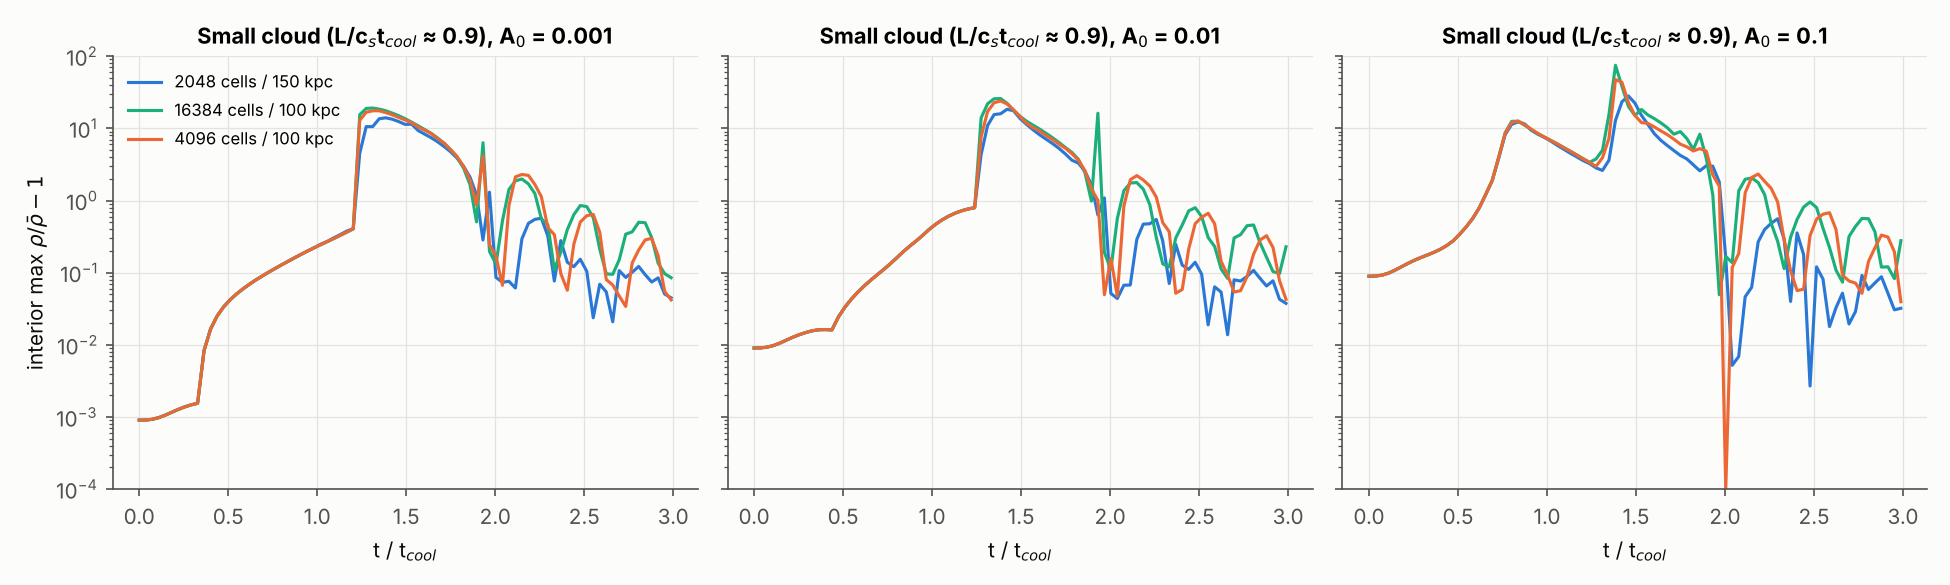
\includegraphics[width=\textwidth]{fig10_resolution.png}
\caption{Interior maximum of $\rho/\bar\rho-1$ for the small cloud at three
resolutions and three seed amplitudes.}
\label{fig:resolution}
\end{figure}

\subsection{Photoionizing UV background}
\label{sec:uvb}
The UV background suppresses cooling below $\sim10^5$\,K, strongly at low density
(at $n=10^{-4}$ the $10^5$\,K peak is roughly halved and the hydrogen peak near
$2\times10^4$\,K disappears), and replaces the floor by a density-dependent
$\Teq$ (Figure~\ref{fig:coolmodels}). Because $\Teq$ falls with density,
compressed gas is cooler than its surroundings at equilibrium, which makes it
easier to compress than gas held at a fixed floor. The UV background also breaks
the exact density scaling of collisional cooling, though only weakly.

\begin{figure}[H]
\centering
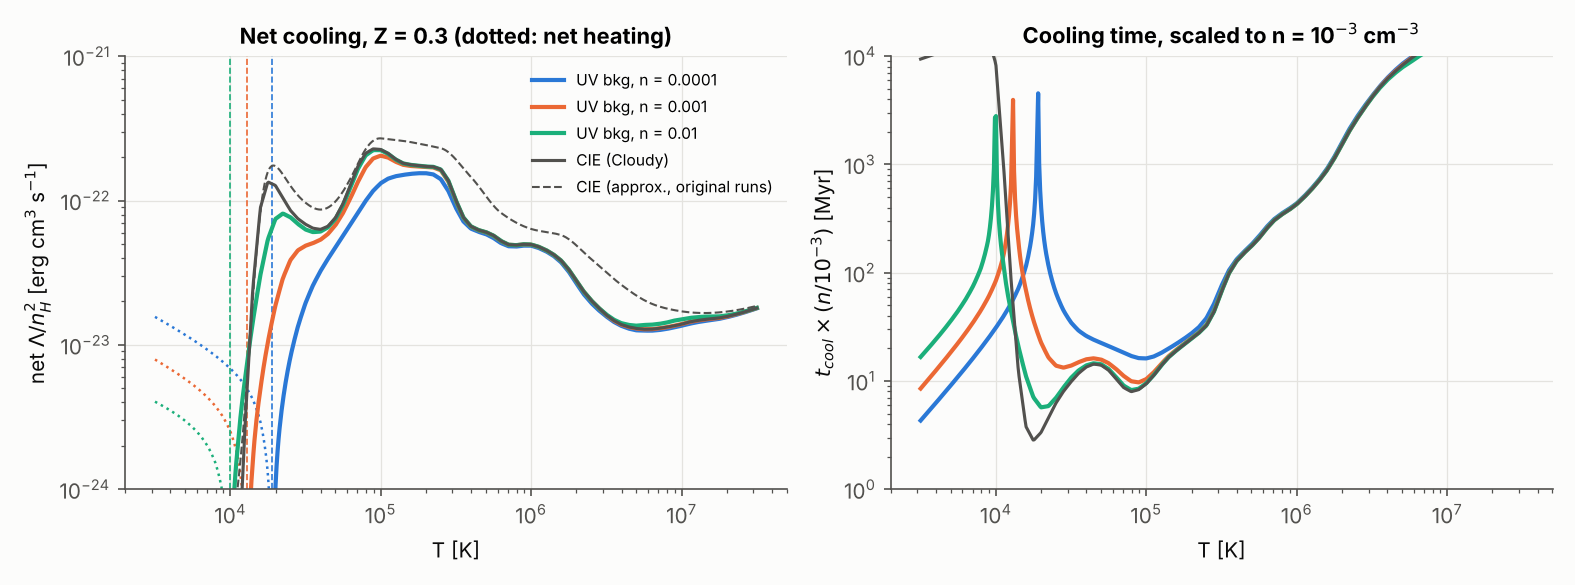
\includegraphics[width=\textwidth]{fig12_cooling_models.png}
\caption{Left: net cooling rate per $n_H^2$ with the UV background at three
densities (dotted: net heating), Cloudy CIE, and the original approximate curve.
Vertical dashed lines mark $\Teq$. Right: cooling time scaled to
$n=10^{-3}$\,cm$^{-3}$.}
\label{fig:coolmodels}
\end{figure}

\begin{figure}[H]
\centering
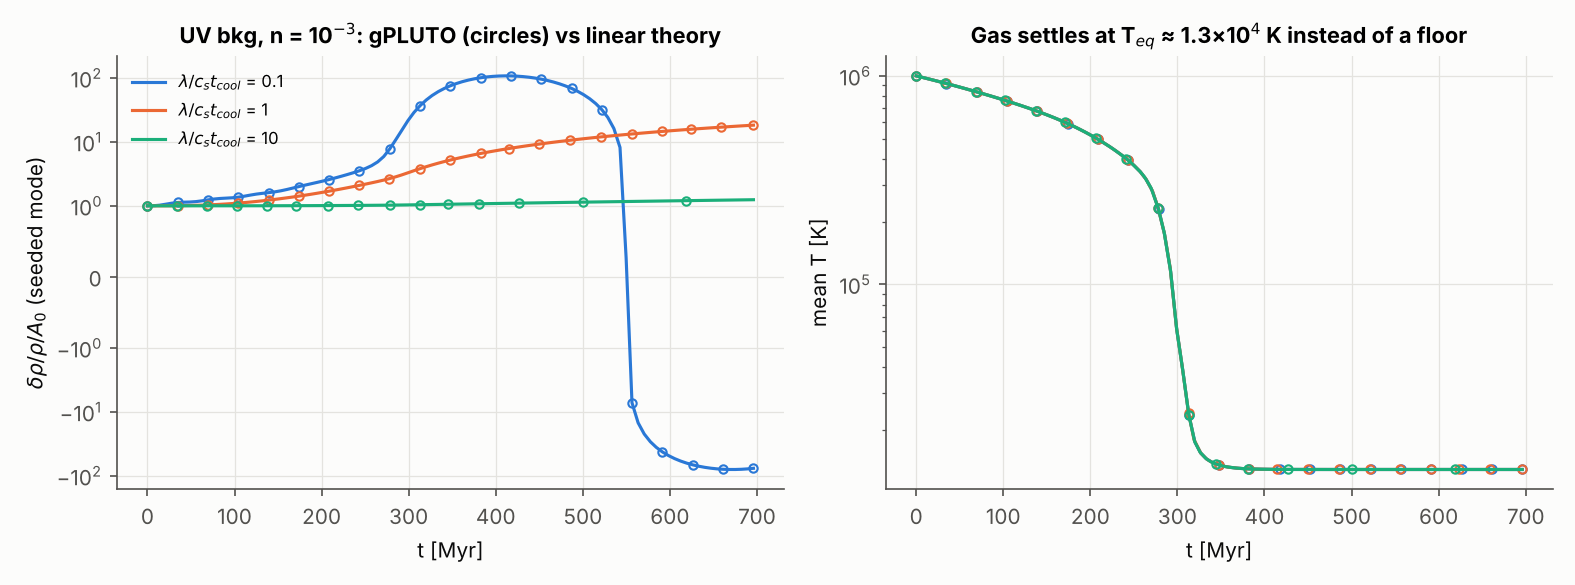
\includegraphics[width=\textwidth]{fig13_validation_uvb.png}
\caption{Validation with the UV background ($n=10^{-3}$\,cm$^{-3}$): gPLUTO
(circles) against linear theory (lines). The gas settles at
$\Teq\approx1.3\times10^4$\,K.}
\label{fig:validationuvb}
\end{figure}

In linear theory (Figure~\ref{fig:linearuvb}) the infinite-medium amplification
with the UV background is within $\sim25\%$ of Cloudy CIE with a floor at every
density from $10^{-4}$ to $10^{-2}$, both while cooling and by $3\,\tcool$. For
small isobaric clouds the totals by $3\,\tcool$ also agree to $\sim25\%$. The
simulations reproduce the linear theory for every model, metallicity and
density (Table~\ref{tab:uvb}, Figure~\ref{fig:infuvb}).

\begin{table}[H]
\centering
\small
\caption{Infinite-medium simulations, $Z=0.3$: growth while cooling / by
$2.5\,\tcool$.}
\label{tab:uvb}
\begin{tabular}{lrrrrr}
\toprule
$x=\lambda/(\cstc)$ & 0.03 & 0.1 & 0.3 & 1 & 3 \\
\midrule
original CIE + floor     & 57/123 & 27/103 & 10/68 & 3.4/20 & 1.3/3.6 \\
Cloudy CIE + floor       & 63/125 & 30/108 & 9.7/60 & 3.6/21 & 1.4/4.1 \\
UV bkg, $n=10^{-4}$      & 66/72  & 41/86  & 13/52 & 4.1/21 & 1.5/4.3 \\
UV bkg, $n=10^{-3}$      & 75/109 & 37/107 & 11/62 & 3.8/21 & 1.4/4.1 \\
UV bkg, $n=10^{-2}$      & 82/135 & 37/120 & 11/69 & 3.8/21 & 1.4/4.1 \\
\bottomrule
\end{tabular}
\end{table}

\begin{figure}[H]
\centering
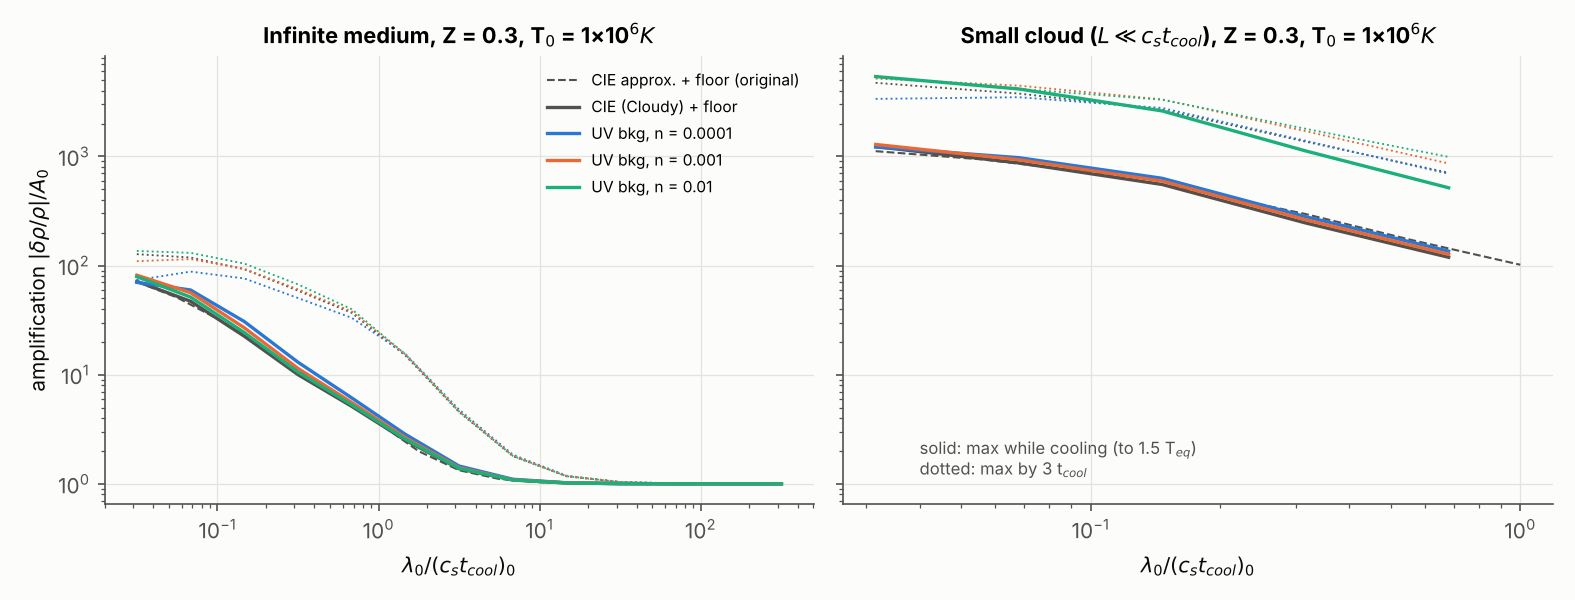
\includegraphics[width=\textwidth]{fig14_linear_uvb.png}
\caption{Linear theory, $Z=0.3$, $T_0=10^6$\,K, for the three cooling models.
Solid: while cooling; dotted: by $3\,\tcool$.}
\label{fig:linearuvb}
\end{figure}

\begin{figure}[H]
\centering
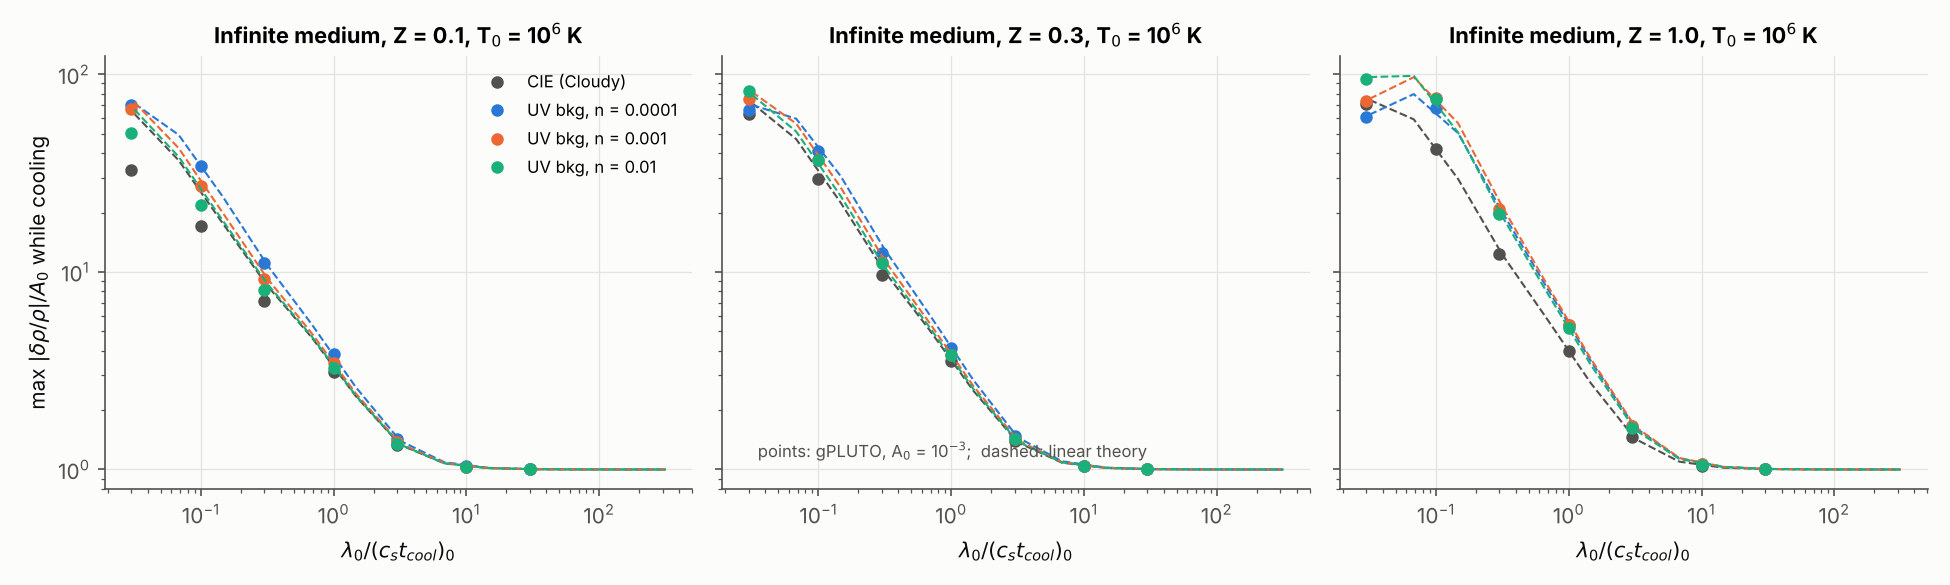
\includegraphics[width=\textwidth]{fig15_infinite_uvb.png}
\caption{Infinite-medium simulations with the Cloudy tables (points) against linear
theory (dashed), for three metallicities.}
\label{fig:infuvb}
\end{figure}

For the 39 cloud pairs resolved in both runs (Figure~\ref{fig:clouduvb}), the
ratio UV/CIE of the growth while cooling has median 1.06 (10--90\%: 1.00--1.78),
and of the growth by $2.5\,\tcool$ 1.32 (1.01--2.37). Equation~(\ref{eq:isoscaling})
holds with the same prefactor (median 24). The main difference is nonlinear
(Figure~\ref{fig:amplitudeuvb}, compared over the same $3\,\tcool$): in the
intermediate cloud ($n_{\rm bg}=10^{-3}$) the UV background makes large seeds go
nonlinear sooner. $A=0.3$ reaches an interior contrast of $\sim100$ by
$1.4\,\tcool$ (CIE + floor: $\sim10$ at $2.5\,\tcool$, $\sim60$ at $3\,\tcool$), and
$A=0.1$ reaches $\sim8$ (CIE + floor: $\sim1$). In the small cloud the transient
structure smooths out more completely ($\sim10^{-3}$ against $\sim0.05$).

\begin{figure}[H]
\centering
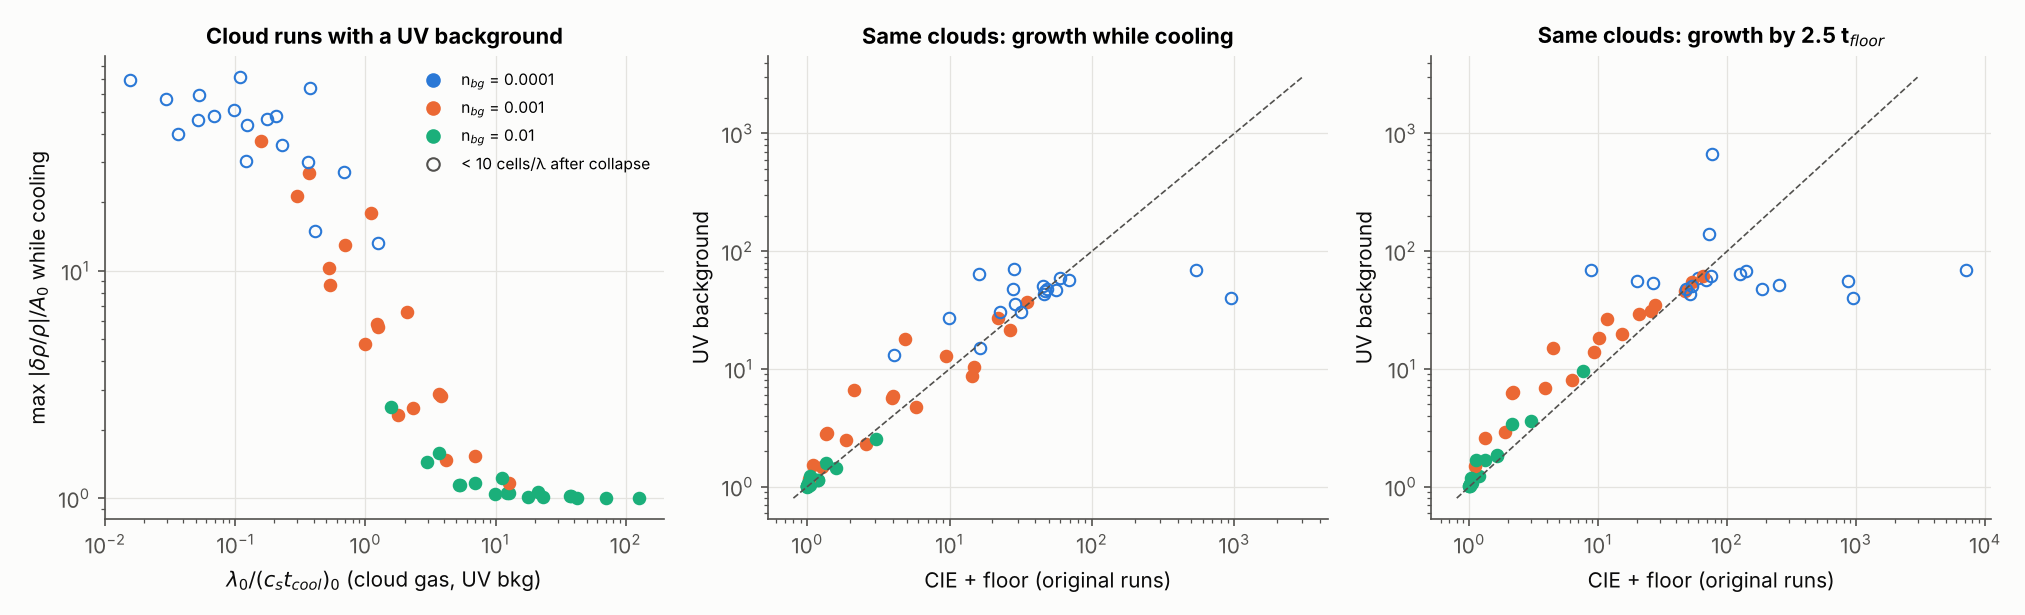
\includegraphics[width=\textwidth]{fig16_cloud_uvb.png}
\caption{Cloud runs with the UV background. Left: growth while cooling against
$x$, coloured by background density; open symbols as in Figure~\ref{fig:clouds}.
Middle and right: the same clouds with the UV background against the original
cooling.}
\label{fig:clouduvb}
\end{figure}

\begin{figure}[H]
\centering
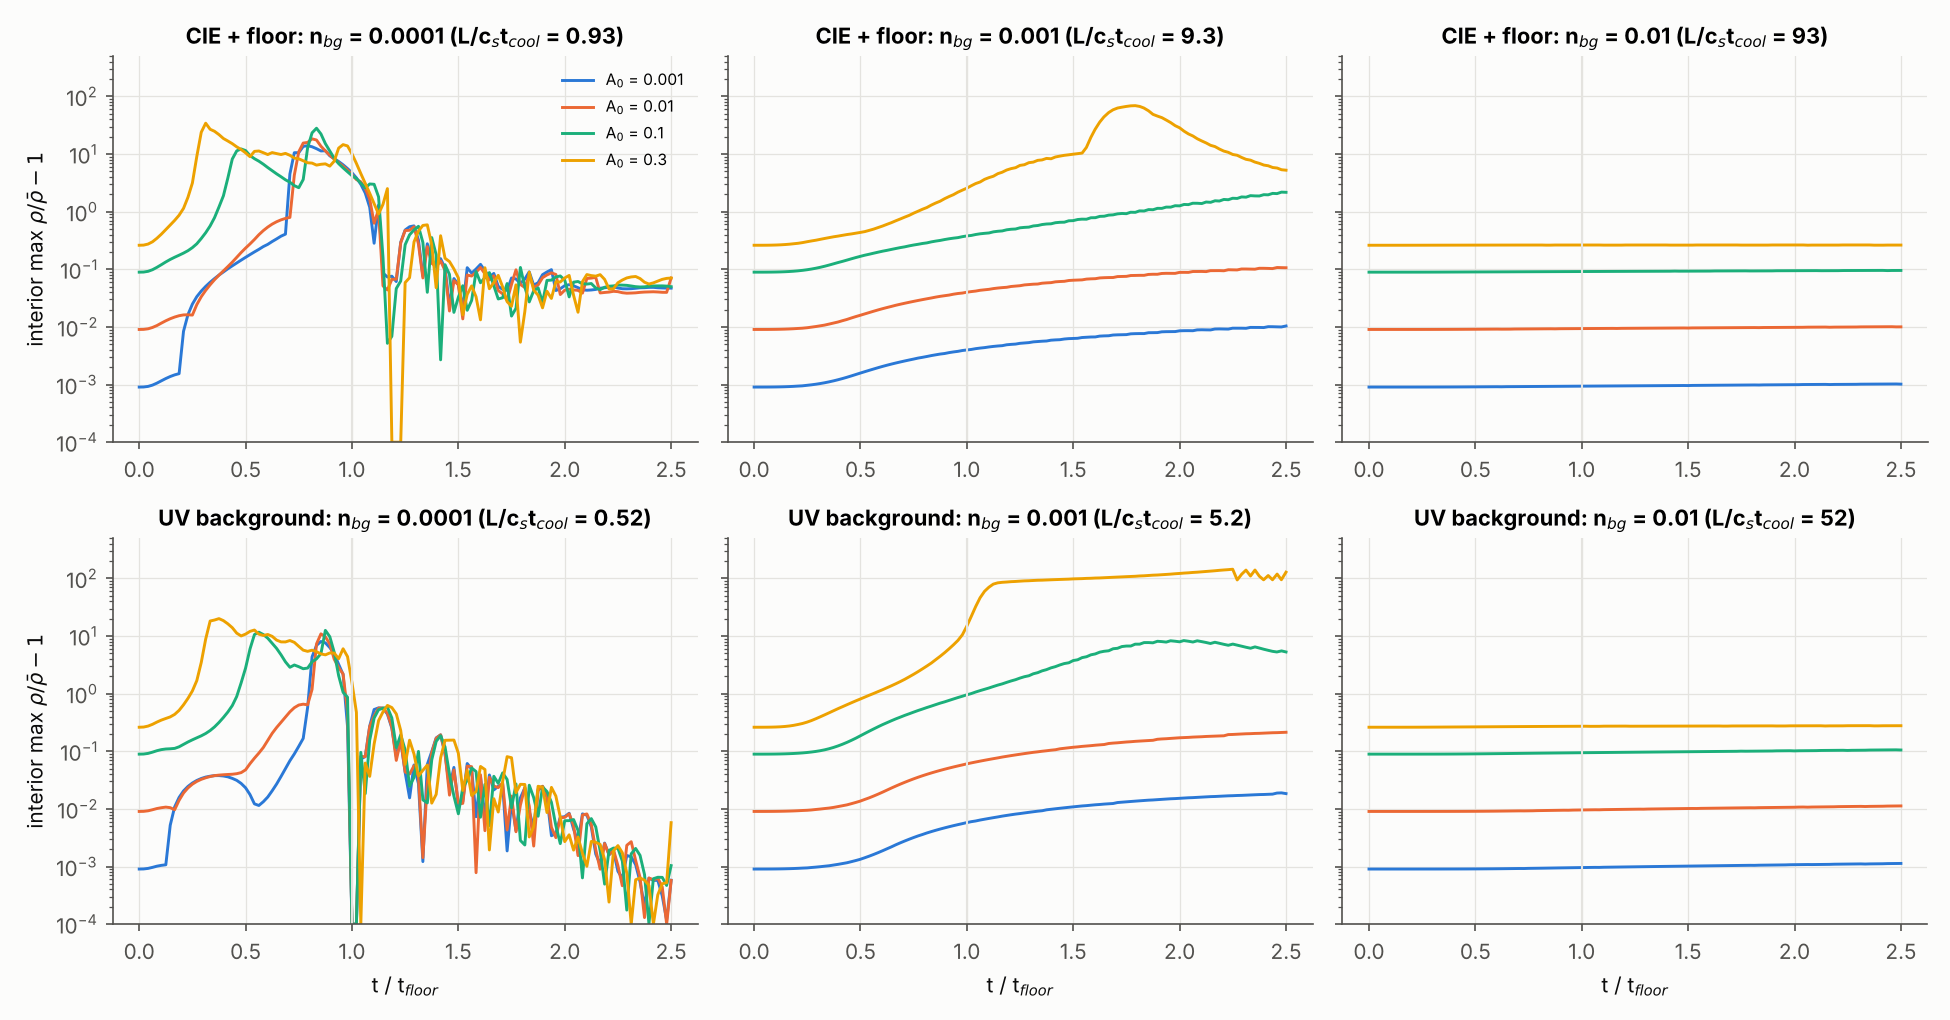
\includegraphics[width=\textwidth]{fig17_amplitude_uvb.png}
\caption{Interior maximum of $\rho/\bar\rho-1$ for four seed amplitudes: collisional
cooling with a floor (top) and the UV background (bottom), at three background
densities.}
\label{fig:amplitudeuvb}
\end{figure}

\subsection{Different kinds of perturbation}
\label{sec:seeds}
Five seeds with the same amplitude $A$ and wavelength (Table~\ref{tab:seeds}).
Metallicity is carried as a second passive tracer, and the cooling uses the Cloudy
primordial and metal rates combined with the local $Z$. These runs use the
Cloudy tables with and without the UV background; the two agree closely (mostly
within 5\%).

\begin{table}[H]
\centering
\small
\caption{Seed types.}
\label{tab:seeds}
\begin{tabular}{lll}
\toprule
seed & initial state & entropy $\delta\ln K$ \\
\midrule
density     & $\drho=A$, $\delta p=0$ (cooler) & $-\gamma A$ \\
temperature & $\delta T/T=\delta p/p=A$, $\delta\rho=0$ (hot spot) & $+A$ \\
sound wave  & $\drho=A$, $\delta p/p=\gamma A$, standing & 0 \\
velocity    & $\delta v=A\,c_s\sin(kx)$ & 0 \\
metallicity & $\delta Z/Z=A$ at uniform $\rho$, $p$ & 0 (but faster cooling) \\
\bottomrule
\end{tabular}
\end{table}

\begin{figure}[H]
\centering
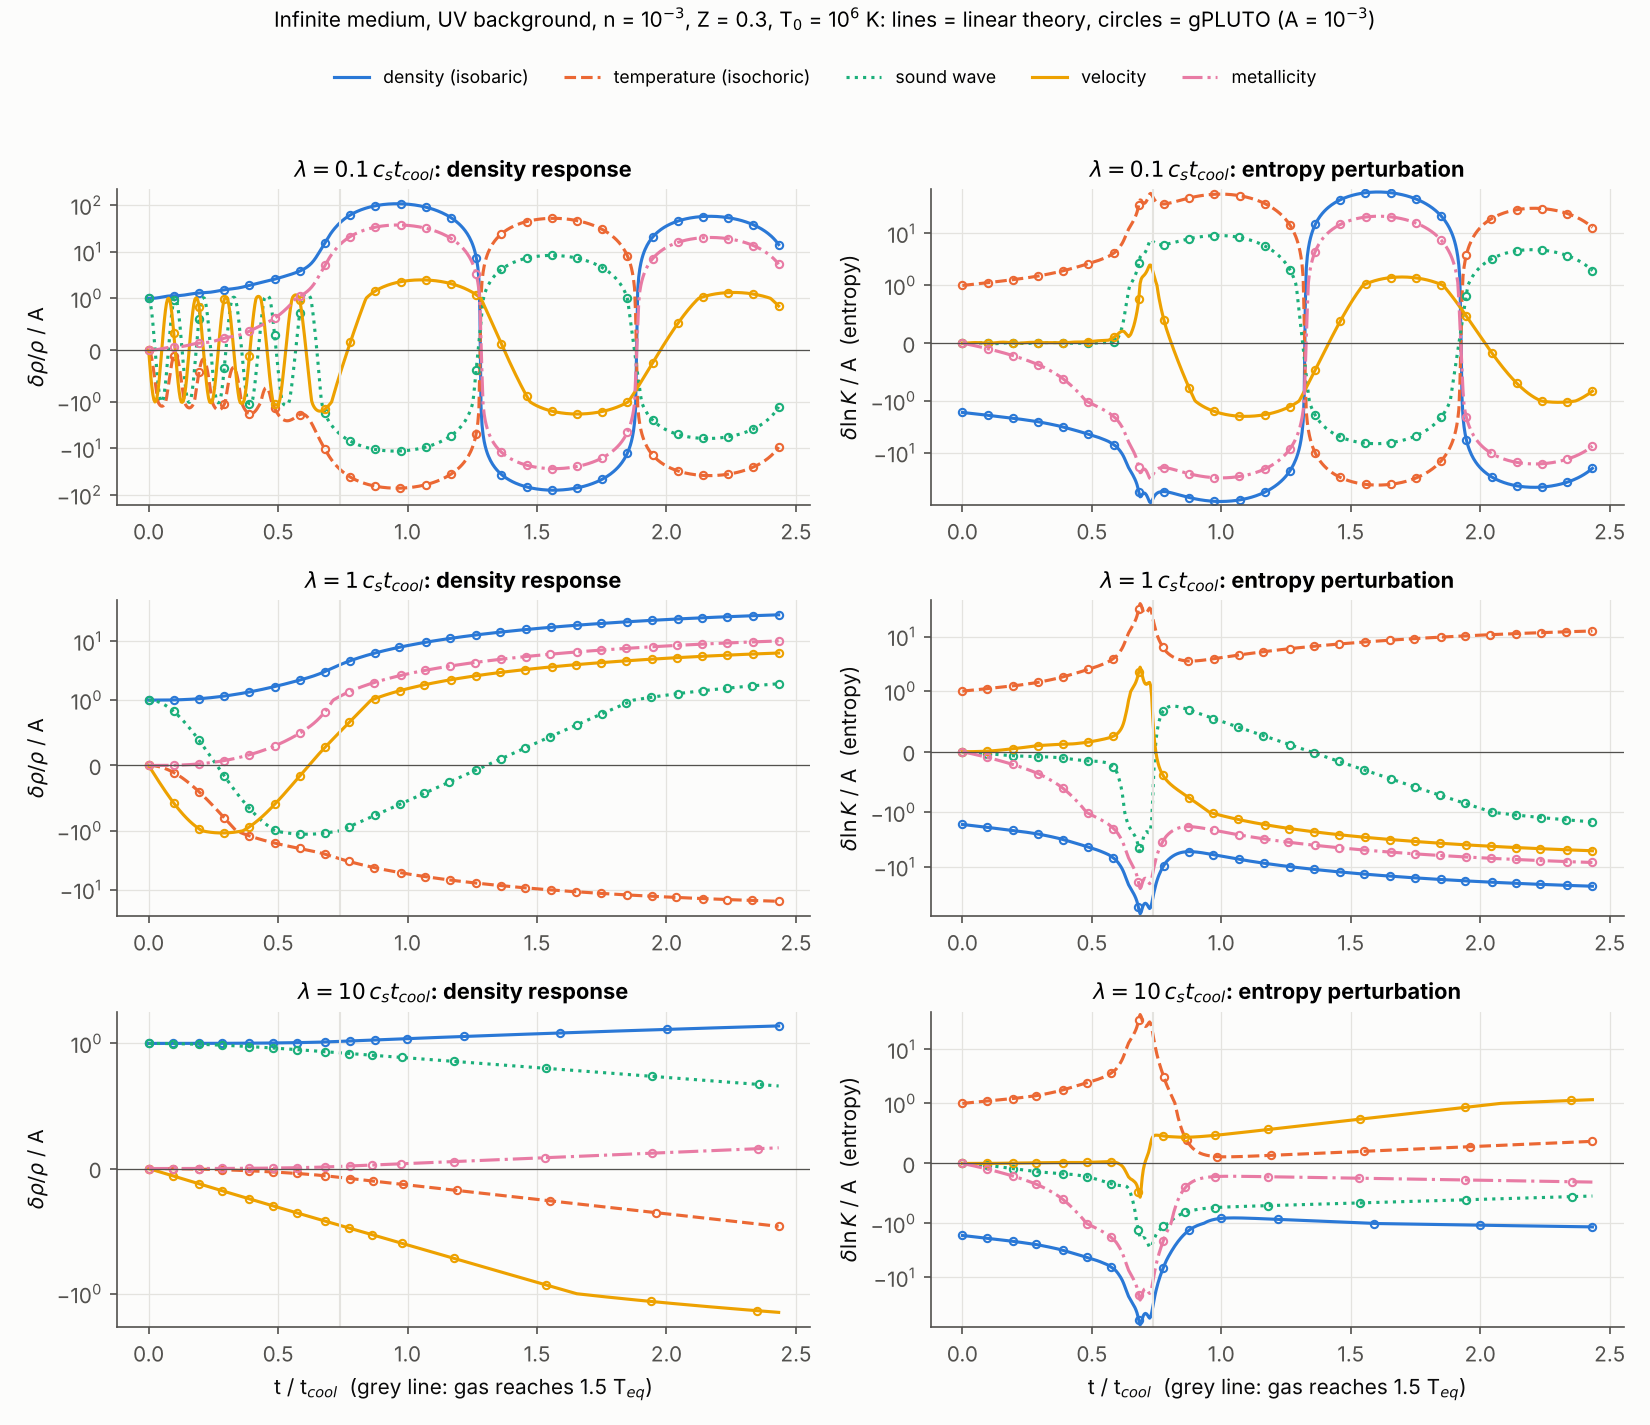
\includegraphics[width=\textwidth]{fig18_pert_histories.png}
\caption{Infinite medium with the UV background, $n=10^{-3}$\,cm$^{-3}$, $Z=0.3$,
$T_0=10^6$\,K: density response (left) and entropy perturbation (right) for the five
seeds, at three wavelengths. Lines: linear theory; circles: gPLUTO ($A=10^{-3}$).}
\label{fig:perthist}
\end{figure}

What grows is the entropy (cooling-time) perturbation
(Table~\ref{tab:seedgrowth}, Figure~\ref{fig:pertlinear}):
\begin{itemize}
\item a \emph{temperature} seed carries $-1/\gamma$ times the entropy perturbation
  of a density seed and gives $\sim0.6$ times its growth, with the opposite sign:
  hot spots end up underdense;
\item a \emph{metallicity} seed changes the cooling rate (metals carry $\sim88\%$
  of the cooling at $10^6$\,K for $Z=0.3$) and gives $\sim0.35$ times the growth of
  a density seed. Metal-rich gas ends up denser, and because $Z$ stays with the
  gas the forcing never switches off;
\item \emph{sound waves} and \emph{velocity} seeds carry no entropy. Cooling
  converts some of their compression into entropy, giving 10--40 times less
  growth than a density seed at short wavelengths. At long wavelengths the
  velocity seed compresses the gas directly and matters about as much as a
  density seed.
\end{itemize}

\begin{table}[H]
\centering
\small
\caption{Growth of the density perturbation, relative to the seed amplitude,
by $3\,\tcool$ (linear theory, infinite medium, $n=10^{-3}$\,cm$^{-3}$, $Z=0.3$).}
\label{tab:seedgrowth}
\begin{tabular}{lrrrrr}
\toprule
$x=\lambda/(\cstc)$ & density & temperature & metallicity & sound & velocity \\
\midrule
$\approx0.15$ & 93  & 50   & 32   & 10  & 8.5--9 \\
$\approx1.5$  & 15  & 11   & 5.3  & 3.8 & 1.5 \\
$\approx15$   & 1.2 & 0.19 & 0.07 & 1.0 & 0.9 \\
\bottomrule
\end{tabular}
\end{table}

\begin{figure}[H]
\centering
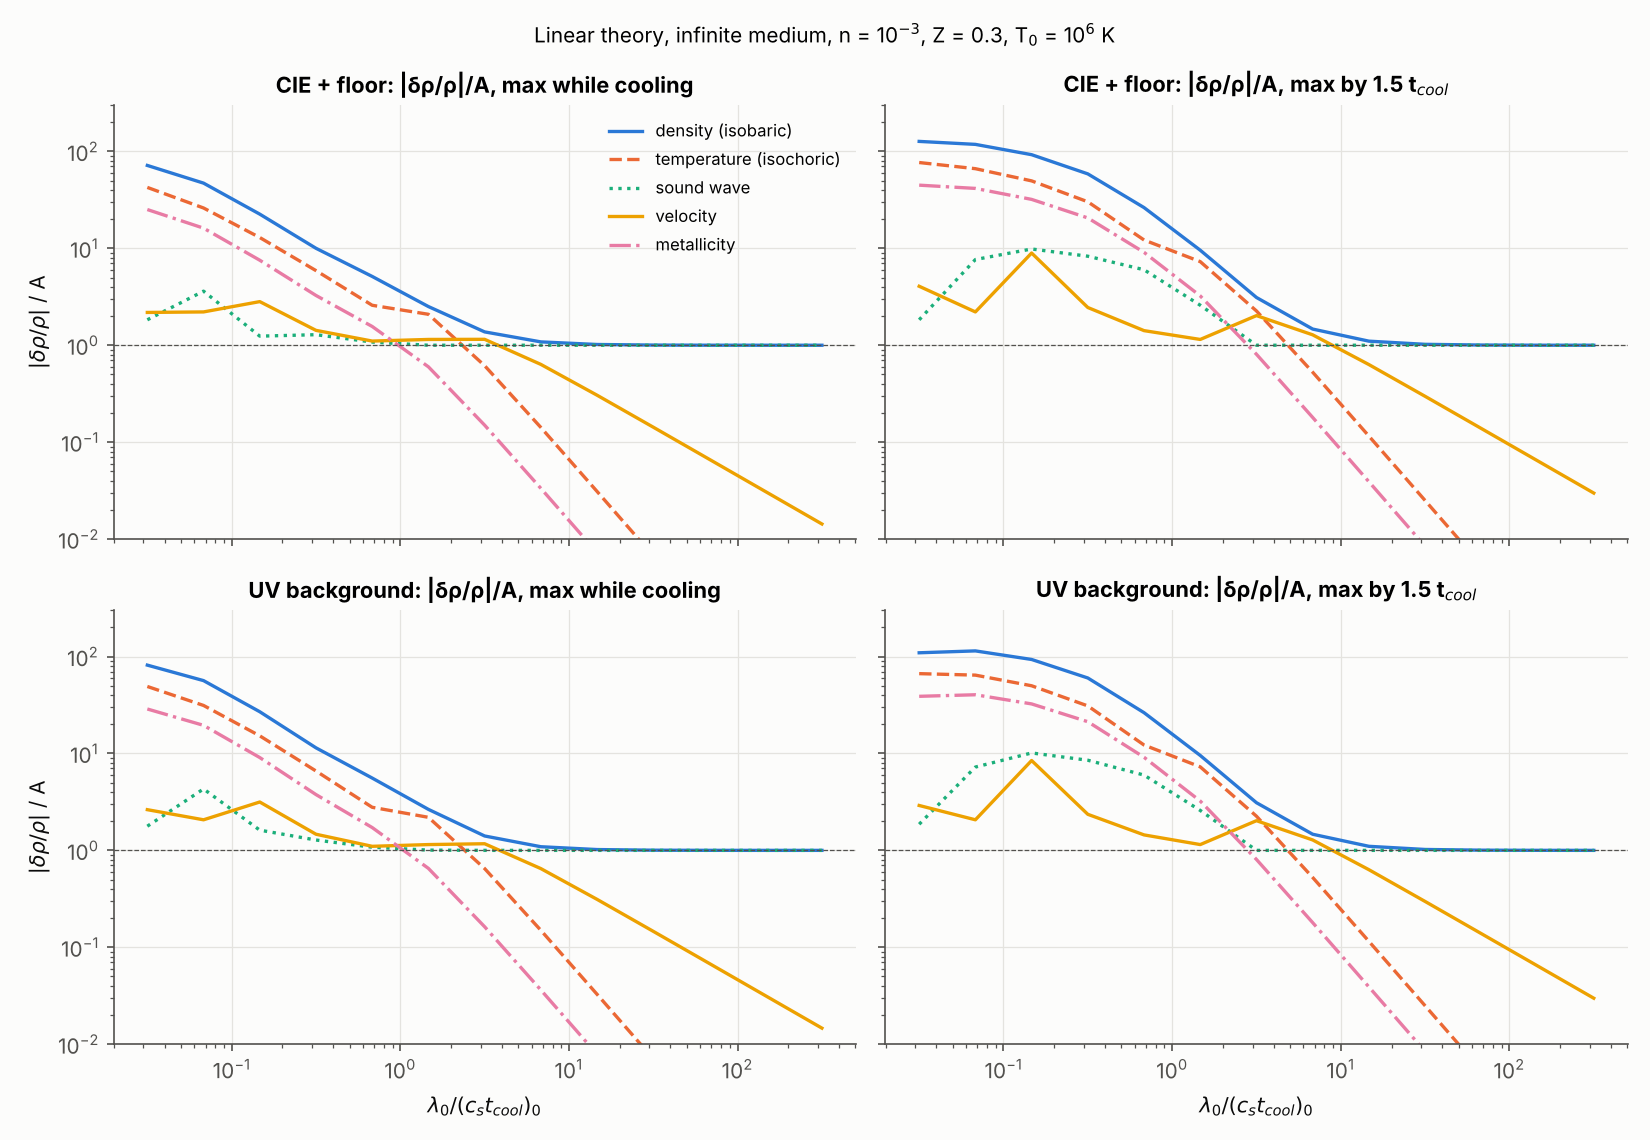
\includegraphics[width=\textwidth]{fig19_pert_linear_survey.png}
\caption{Linear-theory survey of the five seeds against $x$, without (top) and with
(bottom) the UV background. Left: maximum while cooling; right: by $3\,\tcool$.}
\label{fig:pertlinear}
\end{figure}

In clouds ($n_{\rm bg}=10^{-3}$, $x\approx1.2$, $A=0.02$) the ordering is the same:
by $2.5\,\tcool$ the density seed grows 15--16 times, the temperature seed 11--12,
the sound-wave and metallicity seeds $\sim4$ and the velocity seed $\sim3$. At
$n_{\rm bg}=10^{-2}$ ($x\approx12$) only the density seed grows ($\times1.17$);
the others produce at most $0.8A$ (Figure~\ref{fig:pertclouds}). For $A=0.1$ at
$x=0.1$, density, temperature and metallicity seeds condense into clumps 15--34
times denser than the mean, sound waves reach $\sim1.4$ and velocity seeds $\sim0.2$
(Figure~\ref{fig:pertnl}).

\begin{figure}[H]
\centering
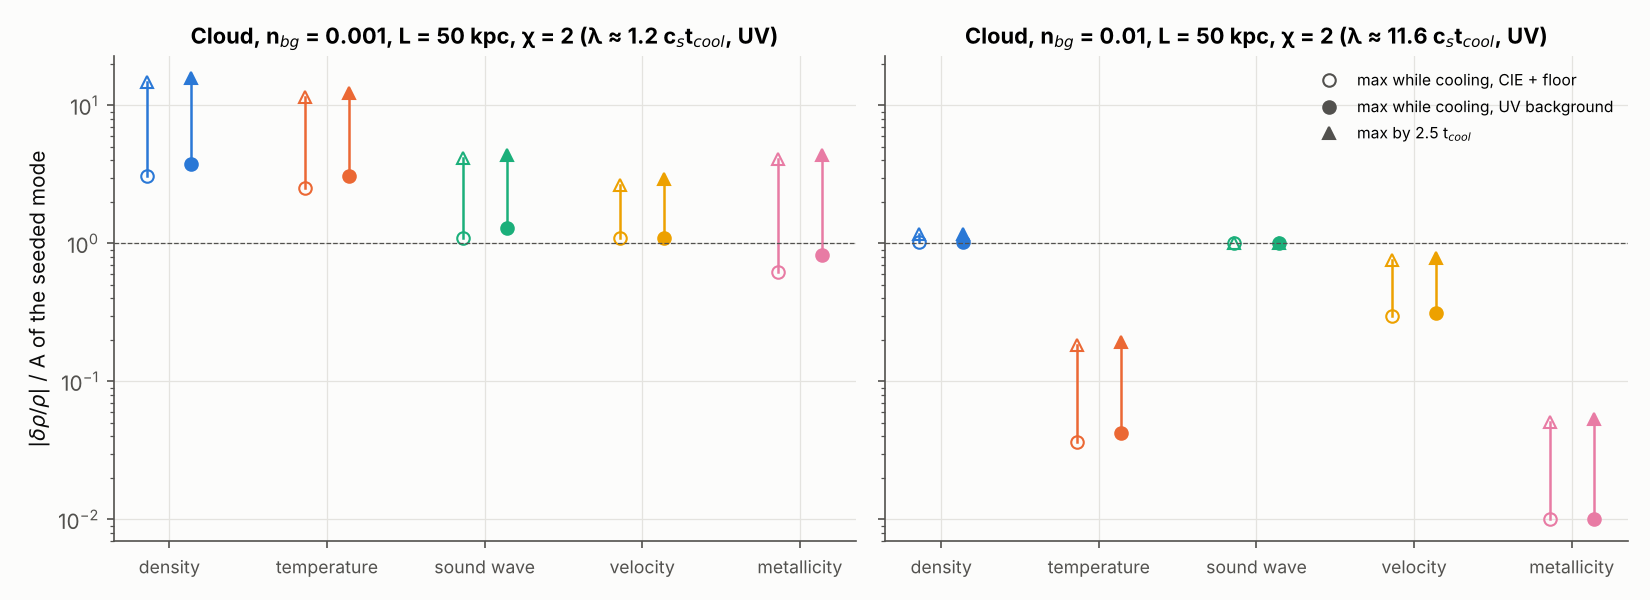
\includegraphics[width=\textwidth]{fig20_pert_clouds.png}
\caption{Cloud runs ($L=50$\,kpc, $\chi=2$, $A=0.02$) for the five seeds. Circles:
maximum while cooling; triangles: maximum by $2.5\,\tcool$. Open: collisional
cooling with a floor; filled: UV background.}
\label{fig:pertclouds}
\end{figure}

\begin{figure}[H]
\centering
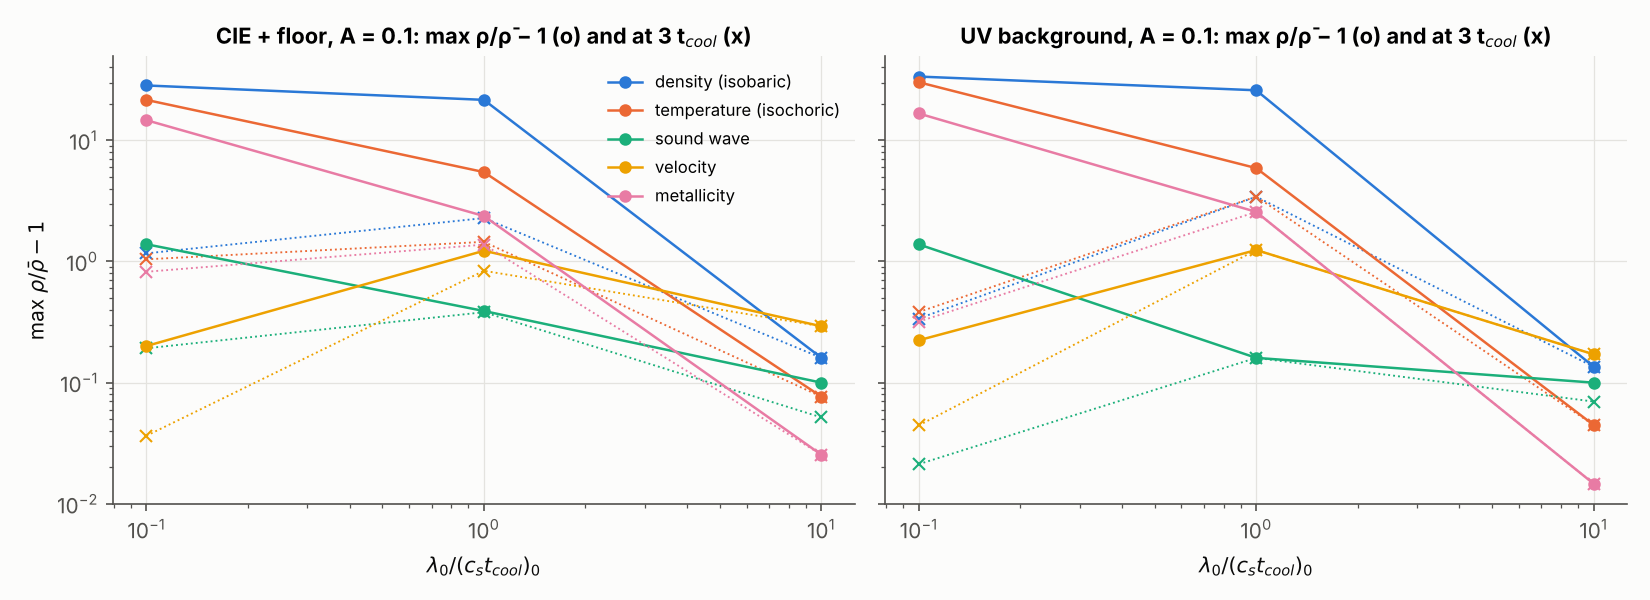
\includegraphics[width=\textwidth]{fig21_pert_nonlinear.png}
\caption{Nonlinear seeds ($A=0.1$), infinite medium: maximum of $\rho/\bar\rho-1$
(circles) and its value at the end of the run (crosses).}
\label{fig:pertnl}
\end{figure}

\subsection{Do perturbations always grow?}
During cooling a density seed never fell below its initial amplitude in any
infinite-medium run starting from $10^5$--$10^6$\,K. In linear theory it can only
shrink where $\LT>2$, which on these curves happens only between about
$2\times10^4$ and $6\times10^4$\,K. Among 320 density-seed simulations, the only
dips (to 0.5--0.86 of the seed) are in five small clouds with just 2.5 wavelengths
per cloud, where motions on the scale of the whole cloud project onto the mode.
After the gas reaches the floor or $\Teq$:
\begin{itemize}
\item at short wavelengths ($x\lesssim0.3$) the perturbation becomes a sound wave in
  the cold gas and swings through zero. With the UV background, residual entropy is
  also erased because gas at $\Teq$ is thermally stable; 10 of 91 infinite-medium and
  14 of 62 cloud runs with the UV background end below their initial amplitude (all
  after first growing more than twofold), against 0 of 63 and 2 of 62 with the floor;
\item small clouds smooth out after collapsing;
\item at $x\gtrsim1$ the post-cooling growth continues through the end of the runs.
\end{itemize}

%======================================================================
\section{Comments on the poster setup}
\label{sec:critique}
%======================================================================
\begin{enumerate}
\item \textbf{Whether the poster's clouds grow depends mostly on $\chi$.} At
  $n_{\rm bg}=0.01$--0.02 and $T_{\rm bg}\approx10^6$\,K, $\cstc$ of the cloud gas is
  0.2--1.4\,kpc for $\chi=2$ but $\sim2$--6\,kpc for $\chi\approx1.3$. With
  $\lambda\approx7$--30\,kpc that is $x\gg1$ for $\chi=2$ but $x\sim2$--5 for
  $\chi\approx1.3$. For $\chi=1.3$, $Z=0.1$, $n_{\rm bg}=0.01$, $L=50$\,kpc we find
  $\times1.8$ while cooling and $\times7$ by $2.5\,\tcool$, the same order as the
  poster's measurements, so her growth looks physical. Most of it comes after the
  gas has cooled. At $\chi=2$ the perturbations still grow, following
  Eq.~(\ref{eq:isoscaling}).
\item \textbf{The diagnostic.} Her central/interior maximum is the right idea.
  Measuring in the mass coordinate (the cloud shrinks) and projecting onto the
  seeded mode (to separate it from harmonics and from waves launched at the edges)
  are two refinements.
\item \textbf{Comparing runs at a fixed simulation time.} $\tcool$ differs by large
  factors between runs. Normalize time by when the gas actually cools
  (Section~\ref{sec:tnorm}), not by when it reaches the floor exactly.
\item \textbf{Use dimensionless parameters}: $\lambda/(\cstc)$, $L/(\cstc)$, $\chi$,
  $Z$ (weakly) and $A$. With collisional cooling, density and size are exactly
  degenerate: runs with $(n,L)=(10^{-2},50\,{\rm kpc})$, $(10^{-3},500\,{\rm kpc})$
  and $(10^{-4},5000\,{\rm kpc})$ agree to 3--4 digits.
\item \textbf{Units and run length.} The poster states 0.1 code units = 0.01\,Gyr,
  but the profiles run to $\sim0.1$\,Gyr; with kpc and 100\,km\,s$^{-1}$ units one
  code time unit is 9.78\,Myr. The runs stop around 1--2\,$\tcool$, before most of
  the post-cooling growth.
\item \textbf{Pressure equilibrium holds only at $t=0$.} Once the cloud cools it
  is out of pressure balance with the hot gas and edge effects reach the interior.
  The periodic infinite medium avoids this.
\item \textbf{Background thermal model.} Switching cooling on only in cloud gas
  works well; a tracer is cleaner than a density threshold (Section~\ref{sec:setup}).
  Uniform heating equal to the background cooling, with cooling everywhere, made the
  shocked hot gas cool into thin radiative shells, and those runs stalled.
\item \textbf{Resolution.} A cloud smaller than $\cstc$ is compressed 50--350 times,
  so cells per wavelength must be counted after the collapse.
\item \textbf{Single sinusoid, single quantity.} The kind of perturbation matters as
  much as its amplitude (Section~\ref{sec:seeds}). A spectrum with random phases in
  several fields is the natural next step.
\item \textbf{Cooling at low density.} A UV background is the better default for CGM
  densities, although it changes the linear results only modestly.
\item \textbf{1D limits.} Cold gas can only form slabs, and at a uniform floor
  temperature and pressure the slabs end at the same density. ``Shattering''
  needs 2D or 3D; the 1D survey tells you which ($x$, $L/\cstc$, $A$, seed type) to
  run there.
\end{enumerate}

\section{Suggested next steps}
\begin{enumerate}
\item Reproduce Figure~\ref{fig:validation} with the student's own PLUTO install,
  to validate the code, cooling table and diagnostic.
\item Make the central plot amplification against $\lambda/(\cstc)$ for several
  $L/(\cstc)$ with linear theory and simulations together (Figure~\ref{fig:clouds}),
  then the minimum-amplitude map (Figure~\ref{fig:minamp}) and the seed comparison
  (Figure~\ref{fig:pertlinear}).
\item Run longer ($\gtrsim5\,\tcool$) to see where the post-cooling growth saturates,
  then follow the nonlinear outcome for $x\lesssim1$ and $A\gtrsim0.01$ at higher
  resolution and in 2D.
\end{enumerate}

\section{Limitations}
\begin{itemize}
\item The original cooling curve is an approximation (0.1--0.3\,dex off between
  $2\times10^5$ and $3\times10^6$\,K); the Cloudy runs give the same trends.
\item The UV-background runs use $z=0$ only, keep the mean molecular weight of fully
  ionized gas (so $T$ is slightly misplaced near $10^4$\,K), and ignore self-shielding.
\item The PLUTO~4.4 port of the setup in the repository was not compiled.
\item Late-time values for strongly compressed small clouds are resolution-limited
  (Section~\ref{sec:resolution}).
\end{itemize}

\appendix
\section{Corrections to earlier versions}
\label{app:corrections}
\begin{itemize}
\item \textbf{Time normalization.} Earlier versions ended ``cooling'' when the gas
  reached $1.05\,\Tfl$ or $1.05\,\Teq$. With the corrected definition the growth
  while cooling is about two times smaller at $x\lesssim0.3$, the prefactor of
  Eq.~(\ref{eq:isoscaling}) is 25 rather than 50, and the $\chi=1.3$ example gives
  $\times1.8$ and $\times7$ rather than $\times3$ and $\times10$.
\item \textbf{UV background.} An earlier version said the UV background roughly
  halves the growth while cooling at $x\approx0.3$--3. That came from the slow final
  approach to the floor in the Cloudy CIE table inflating its end-of-cooling time;
  with consistent times the two agree to $\sim20\%$.
\item \textbf{Run lengths.} Late-time contrasts were previously compared across runs
  of different length in units of $\tcool$; they are now compared over the same
  $3\,\tcool$.
\item \textbf{Diagnostic.} An early version said the poster's measurement was
  dominated by the cloud edges; the student measures the interior, which is sound.
\end{itemize}

\begin{thebibliography}{99}
\bibitem[Das et al.(2021)]{das21}
Das, H.~K., Choudhury, P.~P., \& Sharma, P. 2021, MNRAS, 502, 4935
\bibitem[Haardt \& Madau(2012)]{hm12}
Haardt, F., \& Madau, P. 2012, ApJ, 746, 125
\bibitem[Katz et al.(1996)]{katz96}
Katz, N., Weinberg, D.~H., \& Hernquist, L. 1996, ApJS, 105, 19
\bibitem[McCourt et al.(2018)]{mccourt18}
McCourt, M., Oh, S.~P., O'Leary, R., \& Madigan, A.-M. 2018, MNRAS, 473, 5407
\bibitem[Mignone et al.(2007)]{mignone07}
Mignone, A., Bodo, G., Massaglia, S., et al. 2007, ApJS, 170, 228
\bibitem[Smith et al.(2017)]{smith17}
Smith, B.~D., Bryan, G.~L., Glover, S.~C.~O., et al. 2017, MNRAS, 466, 2217
\bibitem[Sutherland \& Dopita(1993)]{sd93}
Sutherland, R.~S., \& Dopita, M.~A. 1993, ApJS, 88, 253
\end{thebibliography}

\end{document}
